\documentclass[a4paper]{book}
\usepackage{a4wide}
\usepackage{makeidx}
\usepackage{graphicx}
\usepackage{multicol}
\usepackage{float}
\usepackage{listings}
\usepackage{color}
\usepackage{textcomp}
\usepackage{alltt}
\usepackage{times}
\usepackage{ifpdf}
\ifpdf
\usepackage[pdftex,
            pagebackref=true,
            colorlinks=true,
            linkcolor=blue,
            unicode
           ]{hyperref}
\else
\usepackage[ps2pdf,
            pagebackref=true,
            colorlinks=true,
            linkcolor=blue,
            unicode
           ]{hyperref}
\usepackage{pspicture}
\fi
\usepackage[utf8]{inputenc}
\usepackage{doxygen}
\lstset{language=C++,inputencoding=utf8,basicstyle=\footnotesize,breaklines=true,breakatwhitespace=true,tabsize=8,numbers=left }
\makeindex
\setcounter{tocdepth}{3}
\renewcommand{\footrulewidth}{0.4pt}
\begin{document}
\hypersetup{pageanchor=false}
\begin{titlepage}
\vspace*{7cm}
\begin{center}
{\Large JREngage }\\
\vspace*{1cm}
{\large Generated by Doxygen 1.7.1}\\
\vspace*{0.5cm}
{\small Wed Sep 29 2010 19:13:06}\\
\end{center}
\end{titlepage}
\clearemptydoublepage
\pagenumbering{roman}
\tableofcontents
\clearemptydoublepage
\pagenumbering{arabic}
\hypersetup{pageanchor=true}
\chapter{Janrain Engage for the iPhone, version 2}
\label{index}\hypertarget{index}{}\href{http://rpxnow.com/docs/iphone_v2}{\tt Janrain Engage for iPhone} makes it easy to include third party authentication and social publishing in your iPhone app. This Objective-\/C library includes the same key features as our web version. With a few lines of code, you can authenticate your users with their accounts on Google, Yahoo!, Facebook, etc., and they can immediately publish their activities to multiple social networks, including Facebook, Twitter, LinkedIn, MySpace and Yahoo, through one simple interface.

Before you begin, you need to have created a \href{https://rpxnow.com/signup_createapp_plus}{\tt Janrain Engage application}, which you can do on \href{http://rpxnow.com}{\tt http://rpxnow.com}

For an overview of how the library works and how you can take advantage of the library's features, please see the \href{http://rpxnow.com/docs/iphone_v2#user_experience}{\tt \char`\"{}Overview\char`\"{}} section of our documentation.

To begin using the library, please see the \href{http://rpxnow.com/docs/iphone_v2#quick}{\tt \char`\"{}Quick Start Guide\char`\"{}}.

For more detailed documentation of the library's API, you can use the \href{http://rpxnow.com/docs/jrengage_api}{\tt \char`\"{}JREngage API\char`\"{}} documentation. 
\chapter{Providers}
\label{Providers}
\hypertarget{Providers}{}
\hypertarget{_providers_basicProviders}{}\section{List of Providers}\label{_providers_basicProviders}
Here is a list of possible strings that the argument (NSString$\ast$)provider can be when used in the authentication methods:
\begin{DoxyItemize}
\item \char`\"{}aol\char`\"{}
\item \char`\"{}blogger\char`\"{}
\item \char`\"{}facebook\char`\"{}
\item \char`\"{}flickr\char`\"{}
\item \char`\"{}google\char`\"{}
\item \char`\"{}hyves\char`\"{}
\item \char`\"{}linkedin\char`\"{}
\item \char`\"{}live\_\-id\char`\"{}
\item \char`\"{}livejournal\char`\"{}
\item \char`\"{}myopenid\char`\"{}
\item \char`\"{}myspace\char`\"{}
\item \char`\"{}netlog\char`\"{}
\item \char`\"{}openid\char`\"{}
\item \char`\"{}twitter\char`\"{}
\item \char`\"{}verisign\char`\"{}
\item \char`\"{}wordpress\char`\"{}
\item \char`\"{}yahoo\char`\"{}
\end{DoxyItemize}

\begin{DoxyNote}{Note}
As your Engage application is limited by the number of providers it may use, you may only see a subset of this list.
\end{DoxyNote}
\hypertarget{_providers_socialProviders}{}\section{List of Social Providers}\label{_providers_socialProviders}
Here is a list of possible strings that the argument (NSString$\ast$)provider can be when used in the social publishing methods:
\begin{DoxyItemize}
\item \char`\"{}facebook\char`\"{}
\item \char`\"{}linkedin\char`\"{}
\item \char`\"{}myspace\char`\"{}
\item \char`\"{}twitter\char`\"{}
\item \char`\"{}yahoo\char`\"{}
\end{DoxyItemize}

\begin{DoxyNote}{Note}
As your Engage application is limited by the number of providers it may use, you may only see a subset of this list. 
\end{DoxyNote}

\chapter{Class Index}
\section{Class List}
Here are the classes, structs, unions and interfaces with brief descriptions:\begin{DoxyCompactList}
\item\contentsline{section}{\hyperlink{interface_j_r_action_link}{JRActionLink} (A link a user can use to take action on an activity update on the provider )}{\pageref{interface_j_r_action_link}}{}
\item\contentsline{section}{\hyperlink{interface_j_r_activity_object}{JRActivityObject} (An activity object you create, populate, and post to the user's activity stream )}{\pageref{interface_j_r_activity_object}}{}
\item\contentsline{section}{\hyperlink{interface_j_r_engage}{JREngage} (Main API for interacting with the Janrain Engage for iPhone library )}{\pageref{interface_j_r_engage}}{}
\item\contentsline{section}{\hyperlink{protocol_j_r_engage_delegate-p}{$<$JREngageDelegate$>$} (The \hyperlink{protocol_j_r_engage_delegate-p}{JREngageDelegate} protocol is adopted by an object that wishes to receive notifications when and information about a user that authenticates with your application and publishes activities to their social networks )}{\pageref{protocol_j_r_engage_delegate-p}}{}
\item\contentsline{section}{\hyperlink{interface_j_r_flash_media_object}{JRFlashMediaObject} (Flash object to be included in a post to a user's stream )}{\pageref{interface_j_r_flash_media_object}}{}
\item\contentsline{section}{\hyperlink{interface_j_r_image_media_object}{JRImageMediaObject} (Image object to be included in a post to a user's stream )}{\pageref{interface_j_r_image_media_object}}{}
\item\contentsline{section}{\hyperlink{interface_j_r_media_object}{JRMediaObject} }{\pageref{interface_j_r_media_object}}{}
\item\contentsline{section}{\hyperlink{interface_j_r_mp3_media_object}{JRMp3MediaObject} (Mp3 object to be included in a post to a user's stream )}{\pageref{interface_j_r_mp3_media_object}}{}
\end{DoxyCompactList}

\chapter{File Index}
\section{File List}
Here is a list of all documented files with brief descriptions:\begin{DoxyCompactList}
\item\contentsline{section}{/Users/lillialexis/iPhone/engage.iphone/JREngage/Classes/\hyperlink{_j_r_activity_object_8h}{JRActivityObject.h} (Interface for creating and populating activities that you wish to publish )}{\pageref{_j_r_activity_object_8h}}{}
\item\contentsline{section}{/Users/lillialexis/iPhone/engage.iphone/JREngage/Classes/{\bfseries JRConnectionManager.h} }{\pageref{_j_r_connection_manager_8h}}{}
\item\contentsline{section}{/Users/lillialexis/iPhone/engage.iphone/JREngage/Classes/{\bfseries JREngage.h} }{\pageref{_j_r_engage_8h}}{}
\item\contentsline{section}{/Users/lillialexis/iPhone/engage.iphone/JREngage/Classes/{\bfseries JRInfoBar.h} }{\pageref{_j_r_info_bar_8h}}{}
\item\contentsline{section}{/Users/lillialexis/iPhone/engage.iphone/JREngage/Classes/{\bfseries JRProvidersController.h} }{\pageref{_j_r_providers_controller_8h}}{}
\item\contentsline{section}{/Users/lillialexis/iPhone/engage.iphone/JREngage/Classes/{\bfseries JRPublishActivityController.h} }{\pageref{_j_r_publish_activity_controller_8h}}{}
\item\contentsline{section}{/Users/lillialexis/iPhone/engage.iphone/JREngage/Classes/{\bfseries JRSessionData.h} }{\pageref{_j_r_session_data_8h}}{}
\item\contentsline{section}{/Users/lillialexis/iPhone/engage.iphone/JREngage/Classes/{\bfseries JRUserInterfaceMaestro.h} }{\pageref{_j_r_user_interface_maestro_8h}}{}
\item\contentsline{section}{/Users/lillialexis/iPhone/engage.iphone/JREngage/Classes/{\bfseries JRUserLandingController.h} }{\pageref{_j_r_user_landing_controller_8h}}{}
\item\contentsline{section}{/Users/lillialexis/iPhone/engage.iphone/JREngage/Classes/{\bfseries JRWebViewController.h} }{\pageref{_j_r_web_view_controller_8h}}{}
\end{DoxyCompactList}

\chapter{Class Documentation}
\hypertarget{interface_j_r_action_link}{
\section{JRActionLink Class Reference}
\label{interface_j_r_action_link}\index{JRActionLink@{JRActionLink}}
}


A link a user can use to take action on an activity update on the provider.  




{\ttfamily \#import $<$JRActivityObject.h$>$}

\subsection*{Properties}
\begin{DoxyCompactItemize}
\item 
NSString $\ast$ \hyperlink{interface_j_r_action_link_a062c02005f1c35e651ffbcab51c50b21}{text}
\item 
NSString $\ast$ \hyperlink{interface_j_r_action_link_a45489781731e5965e20fa66af0bd3072}{href}
\end{DoxyCompactItemize}
\subsection*{Constructors}
\label{_amgrp559a25fdb98a7d1fd1c3771ac568d5e9}
 \begin{DoxyCompactItemize}
\item 
(id) -\/ \hyperlink{interface_j_r_action_link_ae1f056641fd3302efbf23d89452553a5}{initWithText:andHref:}
\item 
(id) + \hyperlink{interface_j_r_action_link_a210a41749ddf22e6ce0a7b797fac2f3f}{actionLinkWithText:andHref:}
\end{DoxyCompactItemize}


\subsection{Detailed Description}
A link a user can use to take action on an activity update on the provider. Create an action link object, fill in the object's fields, and add the object the \hyperlink{interface_j_r_activity_object_aa5c629e1c3b8306b2532ab647f7f6ec5}{JRActivityObject::action\_\-links} array of your \hyperlink{interface_j_r_activity_object}{JRActivityObject}.

Each action link must contain a link, {\itshape href\/}, and some {\itshape text\/}, describing what action will happen if someone clicks the link. Example: 
\begin{DoxyCode}
 action_links: 
 [
   {
     "text": "Rate this quiz result",
     "href": "http://example.com/quiz/12345/result/6789/rate"
   },
   {
     "text": "Take this quiz",
     "href": "http://example.com/quiz/12345/take"
   }
 ]
\end{DoxyCode}
 

\subsection{Member Function Documentation}
\hypertarget{interface_j_r_action_link_ae1f056641fd3302efbf23d89452553a5}{
\index{JRActionLink@{JRActionLink}!initWithText:andHref:@{initWithText:andHref:}}
\index{initWithText:andHref:@{initWithText:andHref:}!JRActionLink@{JRActionLink}}
\subsubsection[{initWithText:andHref:}]{\setlength{\rightskip}{0pt plus 5cm}-\/ (id) initWithText: 
\begin{DoxyParamCaption}
\item[{dummy(NSString $\ast$)}]{ \_\-text}
\item[{andHref:(NSString $\ast$)}]{ \_\-href}
\end{DoxyParamCaption}
}}
\label{interface_j_r_action_link_ae1f056641fd3302efbf23d89452553a5}
Returns a {\ttfamily \hyperlink{interface_j_r_action_link}{JRActionLink}} initialized with the given text and href.


\begin{DoxyParams}{Parameters}
\item[{\em \_\-text}]The text describing the link. This value cannot be {\ttfamily nil}.\item[{\em \_\-imgsrc}]A link a user can use to take action on an activity update on the provider. This value cannot be {\ttfamily nil}.\end{DoxyParams}
\begin{DoxyReturn}{Returns}
A \hyperlink{interface_j_r_action_link}{JRActionLink} initialized with the given text and href. If either {\ttfamily \_\-text} or {\ttfamily \_\-href} are {\itshape nil\/}, returns {\ttfamily nil}. 
\end{DoxyReturn}
\hypertarget{interface_j_r_action_link_a210a41749ddf22e6ce0a7b797fac2f3f}{
\index{JRActionLink@{JRActionLink}!actionLinkWithText:andHref:@{actionLinkWithText:andHref:}}
\index{actionLinkWithText:andHref:@{actionLinkWithText:andHref:}!JRActionLink@{JRActionLink}}
\subsubsection[{actionLinkWithText:andHref:}]{\setlength{\rightskip}{0pt plus 5cm}+ (id) actionLinkWithText: 
\begin{DoxyParamCaption}
\item[{dummy(NSString $\ast$)}]{ \_\-text}
\item[{andHref:(NSString $\ast$)}]{ \_\-href}
\end{DoxyParamCaption}
}}
\label{interface_j_r_action_link_a210a41749ddf22e6ce0a7b797fac2f3f}
Returns a {\ttfamily \hyperlink{interface_j_r_action_link}{JRActionLink}} initialized with the given text and href.


\begin{DoxyParams}{Parameters}
\item[{\em \_\-text}]The text describing the link. This value cannot be {\ttfamily nil}.\item[{\em \_\-imgsrc}]A link a user can use to take action on an activity update on the provider. This value cannot be {\ttfamily nil}.\end{DoxyParams}
\begin{DoxyReturn}{Returns}
A \hyperlink{interface_j_r_action_link}{JRActionLink} initialized with the given text and href. If either {\ttfamily \_\-text} or {\ttfamily \_\-href} are {\itshape nil\/}, returns {\ttfamily nil}. 
\end{DoxyReturn}


\subsection{Properties}
\hypertarget{interface_j_r_action_link_a062c02005f1c35e651ffbcab51c50b21}{
\index{JRActionLink@{JRActionLink}!text@{text}}
\index{text@{text}!JRActionLink@{JRActionLink}}
\subsubsection[{text}]{\setlength{\rightskip}{0pt plus 5cm}-\/ (NSString $\ast$) text\hspace{0.3cm}{\ttfamily  \mbox{[}read, write, retain\mbox{]}}}}
\label{interface_j_r_action_link_a062c02005f1c35e651ffbcab51c50b21}
The text describing the link \hypertarget{interface_j_r_action_link_a45489781731e5965e20fa66af0bd3072}{
\index{JRActionLink@{JRActionLink}!href@{href}}
\index{href@{href}!JRActionLink@{JRActionLink}}
\subsubsection[{href}]{\setlength{\rightskip}{0pt plus 5cm}-\/ (NSString $\ast$) href\hspace{0.3cm}{\ttfamily  \mbox{[}read, write, retain\mbox{]}}}}
\label{interface_j_r_action_link_a45489781731e5965e20fa66af0bd3072}
A link a user can use to take action on an activity update on the provider 

The documentation for this class was generated from the following file:\begin{DoxyCompactItemize}
\item 
/Users/lillialexis/iPhone/engage.iphone/JREngage/Classes/\hyperlink{_j_r_activity_object_8h}{JRActivityObject.h}\end{DoxyCompactItemize}

\hypertarget{interface_j_r_activity_object}{
\section{JRActivityObject Class Reference}
\label{interface_j_r_activity_object}\index{JRActivityObject@{JRActivityObject}}
}


An activity object you create, populate, and post to the user's activity stream.  




{\ttfamily \#import $<$JRActivityObject.h$>$}

\subsection*{Properties}
\begin{Indent}{\bf }\par
{\em \label{_amgrpd41d8cd98f00b204e9800998ecf8427e}
 The various properties of the \hyperlink{interface_j_r_activity_object}{JRActivityObject} that you can configure }\begin{DoxyCompactItemize}
\item 
NSString $\ast$ \hyperlink{interface_j_r_activity_object_ac7f87878433a7d69fc5c8677fc317d6a}{action}
\item 
NSString $\ast$ \hyperlink{interface_j_r_activity_object_a113d240b8b15e625fb0005fbffd00c17}{url}
\item 
NSString $\ast$ \hyperlink{interface_j_r_activity_object_a965d03730324bcda4374450ad648505b}{user\_\-generated\_\-content}
\item 
NSString $\ast$ \hyperlink{interface_j_r_activity_object_ae64ba976e73c3926a04c46ba0aeba583}{title}
\item 
NSString $\ast$ \hyperlink{interface_j_r_activity_object_a35d4fcb4e1aaa9d6325333228104604f}{description}
\item 
NSMutableArray $\ast$ \hyperlink{interface_j_r_activity_object_aa5c629e1c3b8306b2532ab647f7f6ec5}{action\_\-links}
\item 
NSMutableArray $\ast$ \hyperlink{interface_j_r_activity_object_a2e4ff78f83d0f353f8e0c17ed48ce0ab}{media}
\item 
NSMutableDictionary $\ast$ \hyperlink{interface_j_r_activity_object_a1acf84854d275510685a1f2066061c4e}{properties}
\item 
\hyperlink{interface_j_r_email_object}{JREmailObject} $\ast$ \hyperlink{interface_j_r_activity_object_aa26818070a5987c70ef14700d6f6c72c}{email}
\item 
\hyperlink{interface_j_r_sms_object}{JRSmsObject} $\ast$ \hyperlink{interface_j_r_activity_object_a7719b59135bd02dbd03d4b35b17cb0a0}{sms}
\end{DoxyCompactItemize}
\end{Indent}
\subsection*{Constructors}
\label{_amgrp559a25fdb98a7d1fd1c3771ac568d5e9}
 \begin{DoxyCompactItemize}
\item 
(id) -\/ \hyperlink{interface_j_r_activity_object_a61195dc95162d1136d41af3a5f15fe2d}{initWithAction:andUrl:}
\item 
(id) + \hyperlink{interface_j_r_activity_object_a7bfe16e0799ff6c07548ef8aeb778a51}{activityObjectWithAction:andUrl:}
\end{DoxyCompactItemize}


\subsection{Detailed Description}
Create an activity object, fill in the object's fields, and pass the object to the \hyperlink{interface_j_r_engage}{JREngage} library when you are ready to publish. Currently supported providers are:
\begin{DoxyItemize}
\item Facebook
\item LinkedIn
\item Twitter
\item MySpace
\item Yahoo!
\end{DoxyItemize}

Janrain Engage will make a best effort to use all of the fields submitted in the activity request, but note that how they get presented (and which ones are used) ultimately depends on the provider.

This API will work if and only if:
\begin{DoxyItemize}
\item Your Janrain Engage application has been configured with the given provider
\item The user has already authenticated and has given consent to publish activity
\end{DoxyItemize}

Otherwise, you will be given an error response indicating what was wrong. Detailed error responses will also be given if the activity parameter does not meet the formatting requirements described below.

\begin{DoxySeeAlso}{See also}
For more information of Janrain Engage's activity api, see \href{https://rpxnow.com/docs#api_activity}{\tt the activity section} of our API Documentation. 
\end{DoxySeeAlso}


\subsection{Member Function Documentation}
\hypertarget{interface_j_r_activity_object_a61195dc95162d1136d41af3a5f15fe2d}{
\index{JRActivityObject@{JRActivityObject}!initWithAction:andUrl:@{initWithAction:andUrl:}}
\index{initWithAction:andUrl:@{initWithAction:andUrl:}!JRActivityObject@{JRActivityObject}}
\subsubsection[{initWithAction:andUrl:}]{\setlength{\rightskip}{0pt plus 5cm}-\/ (id) initWithAction: 
\begin{DoxyParamCaption}
\item[{dummy(NSString $\ast$)}]{ \_\-action}
\item[{andUrl:(NSString $\ast$)}]{ \_\-url}
\end{DoxyParamCaption}
}}
\label{interface_j_r_activity_object_a61195dc95162d1136d41af3a5f15fe2d}
Returns a {\ttfamily \hyperlink{interface_j_r_activity_object}{JRActivityObject}} initialized with the given action and url.


\begin{DoxyParams}{Parameters}
\item[{\em \_\-action}]A string describing what the user did, written in the third person. This value cannot be {\ttfamily nil}.\item[{\em \_\-url}]The URL of the resource being mentioned in the activity update. This value cannot be {\ttfamily nil}.\end{DoxyParams}
\begin{DoxyReturn}{Returns}
A \hyperlink{interface_j_r_activity_object}{JRActivityObject} initialized with the given action and url. If either {\ttfamily \_\-action} or {\ttfamily \_\-url} are {\itshape nil\/}, returns {\ttfamily nil}. 
\end{DoxyReturn}
\hypertarget{interface_j_r_activity_object_a7bfe16e0799ff6c07548ef8aeb778a51}{
\index{JRActivityObject@{JRActivityObject}!activityObjectWithAction:andUrl:@{activityObjectWithAction:andUrl:}}
\index{activityObjectWithAction:andUrl:@{activityObjectWithAction:andUrl:}!JRActivityObject@{JRActivityObject}}
\subsubsection[{activityObjectWithAction:andUrl:}]{\setlength{\rightskip}{0pt plus 5cm}+ (id) activityObjectWithAction: 
\begin{DoxyParamCaption}
\item[{dummy(NSString $\ast$)}]{ \_\-action}
\item[{andUrl:(NSString $\ast$)}]{ \_\-url}
\end{DoxyParamCaption}
}}
\label{interface_j_r_activity_object_a7bfe16e0799ff6c07548ef8aeb778a51}
Returns a {\ttfamily \hyperlink{interface_j_r_activity_object}{JRActivityObject}} initialized with the given action and url.


\begin{DoxyParams}{Parameters}
\item[{\em \_\-action}]A string describing what the user did, written in the third person. This value cannot be {\ttfamily nil}.\item[{\em \_\-url}]The URL of the resource being mentioned in the activity update. This value cannot be {\ttfamily nil}.\end{DoxyParams}
\begin{DoxyReturn}{Returns}
A \hyperlink{interface_j_r_activity_object}{JRActivityObject} initialized with the given action and url. If either {\ttfamily \_\-action} or {\ttfamily \_\-url} are {\itshape nil\/}, returns {\ttfamily nil}. 
\end{DoxyReturn}


\subsection{Properties}
\hypertarget{interface_j_r_activity_object_ac7f87878433a7d69fc5c8677fc317d6a}{
\index{JRActivityObject@{JRActivityObject}!action@{action}}
\index{action@{action}!JRActivityObject@{JRActivityObject}}
\subsubsection[{action}]{\setlength{\rightskip}{0pt plus 5cm}-\/ (NSString $\ast$) action\hspace{0.3cm}{\ttfamily  \mbox{[}read, assign\mbox{]}}}}
\label{interface_j_r_activity_object_ac7f87878433a7d69fc5c8677fc317d6a}
A string describing what the user did, written in the third person (e.g., \char`\"{}wrote a restaurant review\char`\"{}, \char`\"{}posted a comment\char`\"{}, \char`\"{}took a quiz\char`\"{}) \hypertarget{interface_j_r_activity_object_a113d240b8b15e625fb0005fbffd00c17}{
\index{JRActivityObject@{JRActivityObject}!url@{url}}
\index{url@{url}!JRActivityObject@{JRActivityObject}}
\subsubsection[{url}]{\setlength{\rightskip}{0pt plus 5cm}-\/ (NSString $\ast$) url\hspace{0.3cm}{\ttfamily  \mbox{[}read, assign\mbox{]}}}}
\label{interface_j_r_activity_object_a113d240b8b15e625fb0005fbffd00c17}
The URL of the resource being mentioned in the activity update \hypertarget{interface_j_r_activity_object_a965d03730324bcda4374450ad648505b}{
\index{JRActivityObject@{JRActivityObject}!user\_\-generated\_\-content@{user\_\-generated\_\-content}}
\index{user\_\-generated\_\-content@{user\_\-generated\_\-content}!JRActivityObject@{JRActivityObject}}
\subsubsection[{user\_\-generated\_\-content}]{\setlength{\rightskip}{0pt plus 5cm}-\/ (NSString $\ast$) user\_\-generated\_\-content\hspace{0.3cm}{\ttfamily  \mbox{[}read, write, retain\mbox{]}}}}
\label{interface_j_r_activity_object_a965d03730324bcda4374450ad648505b}
A string containing user-\/supplied content, such as a comment or the first paragraph of an article that the user wrote.

\begin{DoxyNote}{Note}
Some providers (Twitter in particular) may truncate this value. 
\end{DoxyNote}
\hypertarget{interface_j_r_activity_object_ae64ba976e73c3926a04c46ba0aeba583}{
\index{JRActivityObject@{JRActivityObject}!title@{title}}
\index{title@{title}!JRActivityObject@{JRActivityObject}}
\subsubsection[{title}]{\setlength{\rightskip}{0pt plus 5cm}-\/ (NSString $\ast$) title\hspace{0.3cm}{\ttfamily  \mbox{[}read, write, retain\mbox{]}}}}
\label{interface_j_r_activity_object_ae64ba976e73c3926a04c46ba0aeba583}
The title of the resource being mentioned in the activity update.

\begin{DoxyNote}{Note}
No length restriction on the status is imposed by Janrain Engage, however Yahoo truncates this value to 256 characters. 
\end{DoxyNote}
\hypertarget{interface_j_r_activity_object_a35d4fcb4e1aaa9d6325333228104604f}{
\index{JRActivityObject@{JRActivityObject}!description@{description}}
\index{description@{description}!JRActivityObject@{JRActivityObject}}
\subsubsection[{description}]{\setlength{\rightskip}{0pt plus 5cm}-\/ (NSString $\ast$) description\hspace{0.3cm}{\ttfamily  \mbox{[}read, write, retain\mbox{]}}}}
\label{interface_j_r_activity_object_a35d4fcb4e1aaa9d6325333228104604f}
A description of the resource mentioned in the activity update \hypertarget{interface_j_r_activity_object_aa5c629e1c3b8306b2532ab647f7f6ec5}{
\index{JRActivityObject@{JRActivityObject}!action\_\-links@{action\_\-links}}
\index{action\_\-links@{action\_\-links}!JRActivityObject@{JRActivityObject}}
\subsubsection[{action\_\-links}]{\setlength{\rightskip}{0pt plus 5cm}-\/ (NSMutableArray $\ast$) action\_\-links\hspace{0.3cm}{\ttfamily  \mbox{[}read, write, retain\mbox{]}}}}
\label{interface_j_r_activity_object_aa5c629e1c3b8306b2532ab647f7f6ec5}
An array of {\ttfamily \hyperlink{interface_j_r_action_link}{JRActionLink}} objects, each having two attributes: text and href. An action link is a link a user can use to take action on an activity update on the provider Example: 
\begin{DoxyCode}
 action_links: 
 [
   {
     "text": "Rate this quiz result",
     "href": "http://example.com/quiz/12345/result/6789/rate"
   },
   {
     "text": "Take this quiz",
     "href": "http://example.com/quiz/12345/take"
   }
 ]
\end{DoxyCode}


\begin{DoxyNote}{Note}
Any objects added to this array that are not of type {\ttfamily \hyperlink{interface_j_r_action_link}{JRActionLink}} will be ignored. 
\end{DoxyNote}
\hypertarget{interface_j_r_activity_object_a2e4ff78f83d0f353f8e0c17ed48ce0ab}{
\index{JRActivityObject@{JRActivityObject}!media@{media}}
\index{media@{media}!JRActivityObject@{JRActivityObject}}
\subsubsection[{media}]{\setlength{\rightskip}{0pt plus 5cm}-\/ (NSMutableArray $\ast$) media\hspace{0.3cm}{\ttfamily  \mbox{[}read, write, retain\mbox{]}}}}
\label{interface_j_r_activity_object_a2e4ff78f83d0f353f8e0c17ed48ce0ab}
An array of objects with base class {\ttfamily JRMediaObject} (i.e., \hyperlink{interface_j_r_image_media_object}{JRImageMediaObject}, \hyperlink{interface_j_r_flash_media_object}{JRFlashMediaObject}, \hyperlink{interface_j_r_mp3_media_object}{JRMp3MediaObject}).

To publish attached media objects with your activity, create the preferred object, populate the object's fields, then add the object to the {\ttfamily media} array. You can attach pictures, videos, and mp3s to your activity, although how the media objects get presented and whether or not they are used, depend on the provider.

If you include more than one media type in the array, \hyperlink{interface_j_r_engage}{JREngage} will choose only one of these types, in this order:
\begin{DoxyEnumerate}
\item image
\item flash
\item mp3
\end{DoxyEnumerate}

Also, any objects added to this array that are not of type {\ttfamily JRMediaObject} will be ignored.

\begin{DoxySeeAlso}{See also}
Media object format and rules are identical to those described on the \href{http://developers.facebook.com/docs/guides/attachments}{\tt Facebook Developer page on Attachments}. 
\end{DoxySeeAlso}
\hypertarget{interface_j_r_activity_object_a1acf84854d275510685a1f2066061c4e}{
\index{JRActivityObject@{JRActivityObject}!properties@{properties}}
\index{properties@{properties}!JRActivityObject@{JRActivityObject}}
\subsubsection[{properties}]{\setlength{\rightskip}{0pt plus 5cm}-\/ (NSMutableDictionary $\ast$) properties\hspace{0.3cm}{\ttfamily  \mbox{[}read, write, retain\mbox{]}}}}
\label{interface_j_r_activity_object_a1acf84854d275510685a1f2066061c4e}
An object with attributes describing properties of the update. An attribute value can be a string or an object with two attributes, text and href. Example: 
\begin{DoxyCode}
   properties: 
   {
       "Time": "05:00",
       "Location": 
       {
           "text": "Portland",
           "href": "http://en.wikipedia.org/wiki/Portland,_Oregon"
       }
   }
\end{DoxyCode}
 \hypertarget{interface_j_r_activity_object_aa26818070a5987c70ef14700d6f6c72c}{
\index{JRActivityObject@{JRActivityObject}!email@{email}}
\index{email@{email}!JRActivityObject@{JRActivityObject}}
\subsubsection[{email}]{\setlength{\rightskip}{0pt plus 5cm}-\/ ({\bf JREmailObject} $\ast$) email\hspace{0.3cm}{\ttfamily  \mbox{[}read, write, retain\mbox{]}}}}
\label{interface_j_r_activity_object_aa26818070a5987c70ef14700d6f6c72c}
\label{interface_j_r_activity_object_activityEmail}
\hypertarget{interface_j_r_activity_object_activityEmail}{}


An object containing the subject and message body of an email, if the user wishes to share via email. \hypertarget{interface_j_r_activity_object_a7719b59135bd02dbd03d4b35b17cb0a0}{
\index{JRActivityObject@{JRActivityObject}!sms@{sms}}
\index{sms@{sms}!JRActivityObject@{JRActivityObject}}
\subsubsection[{sms}]{\setlength{\rightskip}{0pt plus 5cm}-\/ ({\bf JRSmsObject} $\ast$) sms\hspace{0.3cm}{\ttfamily  \mbox{[}read, write, retain\mbox{]}}}}
\label{interface_j_r_activity_object_a7719b59135bd02dbd03d4b35b17cb0a0}
\label{interface_j_r_activity_object_activitySms}
\hypertarget{interface_j_r_activity_object_activitySms}{}


An object containing the message body of an sms, if the user wishes to share via sms. 

The documentation for this class was generated from the following file:\begin{DoxyCompactItemize}
\item 
/Users/lillialexis/iPhone/engage.iphone/JREngage/Classes/\hyperlink{_j_r_activity_object_8h}{JRActivityObject.h}\end{DoxyCompactItemize}

\hypertarget{interface_j_r_engage}{
\section{JREngage Class Reference}
\label{interface_j_r_engage}\index{JREngage@{JREngage}}
}


Main API for interacting with the Janrain Engage for iPhone library.  




{\ttfamily \#import $<$JREngage.h$>$}



Inherits JRSessionDelegate-\/p.

\subsection*{Static Public Member Functions}
\begin{Indent}{\bf Get the JREngage Instance}\par
{\em \label{_amgrp1563bd99b5767462283658c6804d90b3}
 Methods that initialize and return the shared \hyperlink{interface_j_r_engage}{JREngage} instance }\begin{DoxyCompactItemize}
\item 
(\hyperlink{interface_j_r_engage}{JREngage} $\ast$) + \hyperlink{interface_j_r_engage_adb6bf3a6869d83f2bfce0783f128d9e6}{jrEngage}
\item 
(\hyperlink{interface_j_r_engage}{JREngage} $\ast$) + \hyperlink{interface_j_r_engage_a36c199d6384893b1bf42712771af1e8b}{jrEngageWithAppId:andTokenUrl:delegate:}
\end{DoxyCompactItemize}
\end{Indent}
\subsection*{Public Member Functions}
\begin{Indent}{\bf Manage the Delegates}\par
{\em \label{_amgrpf6bb425cb9b7388d33e37d551db6b02e}
 Add/remove delegates that implement the \hyperlink{protocol_j_r_engage_delegate-p}{JREngageDelegate} protocol }\begin{DoxyCompactItemize}
\item 
(void) -\/ \hyperlink{interface_j_r_engage_a18377ffb55f821587e6d38b3489692e8}{addDelegate:}
\item 
(void) -\/ \hyperlink{interface_j_r_engage_ab3f12ac148ea0f6df4d7ff7789cc7c94}{removeDelegate:}
\end{DoxyCompactItemize}
\end{Indent}
\begin{Indent}{\bf Show the JREngage Dialogs}\par
{\em \label{_amgrp345603279e1df04f4a3678e78089b7be}
 \label{interface_j_r_engage_showMethods}
\hypertarget{interface_j_r_engage_showMethods}{}


Methods that display JREngage's dialogs to initiate authentication and social publishing }\begin{DoxyCompactItemize}
\item 
(void) -\/ \hyperlink{interface_j_r_engage_a01ecdff491f91543e18f33d0e565b046}{showAuthenticationDialog}
\item 
(void) -\/ \hyperlink{interface_j_r_engage_ac8e1206be8608fbed548b7ec5f85e6e6}{showAuthenticationDialogWithCustomInterface:}
\item 
(void) -\/ \hyperlink{interface_j_r_engage_afca7b5ab9a57edc1a460aaec882207c4}{showSocialPublishingDialogWithActivity:}
\item 
(void) -\/ \hyperlink{interface_j_r_engage_af5c2aa40f5c45a22f369900d1bd81953}{showSocialPublishingDialogWithActivity:andCustomInterface:}
\end{DoxyCompactItemize}
\end{Indent}
\begin{Indent}{\bf Configure the User Interface}\par
{\em \label{_amgrp94e7ef441fcaa606cadd8cfd8b428e50}
 Methods used to customize the JREngage's user interface }\begin{DoxyCompactItemize}
\item 
(void) -\/ \hyperlink{interface_j_r_engage_a6c704bbff377d20603e6b52bd0ae17f1}{setCustomNavigationController:}
\item 
(void) -\/ \hyperlink{interface_j_r_engage_ab1757bbe9e83255b1b9128c630267fdf}{setCustomInterface:}
\end{DoxyCompactItemize}
\end{Indent}
\begin{Indent}{\bf Management Authenticated Users}\par
{\em \label{_amgrp4247d2361fbfb57c620ed69782a50c95}
 Methods that manage authenticated users remembered by the library }\begin{DoxyCompactItemize}
\item 
(void) -\/ \hyperlink{interface_j_r_engage_aede9ed92d80f14d85e59a982da3150fc}{signoutUserForSocialProvider:}
\item 
(void) -\/ \hyperlink{interface_j_r_engage_a1f4e27ed5dbc05892fd7bc2255d2afa8}{signoutUserForAllSocialProviders}
\item 
(void) -\/ \hyperlink{interface_j_r_engage_af1448791663265d3b739041983fbae92}{signoutUserForProvider:}
\item 
(void) -\/ \hyperlink{interface_j_r_engage_a56060e8d5fe94e4bf06ff3edf27af5ee}{signoutUserForAllProviders}
\item 
(void) -\/ \hyperlink{interface_j_r_engage_a66dca1abdfd5103480f9a87f65923a68}{alwaysForceReauthentication:}
\end{DoxyCompactItemize}
\end{Indent}
\begin{Indent}{\bf Cancel the JREngage Dialogs}\par
{\em \label{_amgrpd07ee85d05cc5dd13dd0e31682479a39}
 Methods to cancel authentication and social publishing }\begin{DoxyCompactItemize}
\item 
(void) -\/ \hyperlink{interface_j_r_engage_a17b67c9bb98230fb7d59f8c35a20662b}{cancelAuthentication}
\item 
(void) -\/ \hyperlink{interface_j_r_engage_a205c368338061976178a5b0e36f2d4f2}{cancelPublishing}
\end{DoxyCompactItemize}
\end{Indent}
\begin{Indent}{\bf Server-\/side Authentication}\par
{\em \label{_amgrp1fc6cae7bdf84f91a0bad45f5891f15e}
 Methods to reconfigure server-\/side authentication }\begin{DoxyCompactItemize}
\item 
(void) -\/ \hyperlink{interface_j_r_engage_ac0fb45ee43767dfdea0057bb93000db6}{updateTokenUrl:}
\end{DoxyCompactItemize}
\end{Indent}


\subsection{Detailed Description}
Main API for interacting with the Janrain Engage for iPhone library. Use the \hyperlink{interface_j_r_engage}{JREngage} object to authenticate a user with your application and allow them to publish activities to their social networks.

If you wish to include 3rd-\/Party Authentication and Social Publishing in your iPhone application, you can use the \hyperlink{interface_j_r_engage}{JREngage} class to achieve this. Prior to using the \hyperlink{interface_j_r_engage}{JREngage} library, you must already have an application on \href{http://rpxnow.com}{\tt http://rpxnow.com}. This is all that is required for basic authentication, although some providers may require extra configuration (which can be done through your application's \href{http://rpxnow.com/relying_parties}{\tt Dashboard} For social publishing, you will need to configure your rpxnow application with the desired providers.

If desired, you can optionally implement server-\/side authentication$\ast$. When provided, the \hyperlink{interface_j_r_engage}{JREngage} library can post the user's authentication token to a url on your server: the token url. Your server can complete authentication, access more of JREngage's API, log the authentication, etc. and the server's response will be passed back through to your iPhone application.

$\ast$In the previous version of the Engage for iPhone library, implementing token url that completed server-\/side authentication was required. This is no longer the case, although you can optionally implement the token url if you wish to continue authentication on your server. 

\subsection{Member Function Documentation}
\hypertarget{interface_j_r_engage_adb6bf3a6869d83f2bfce0783f128d9e6}{
\index{JREngage@{JREngage}!jrEngage@{jrEngage}}
\index{jrEngage@{jrEngage}!JREngage@{JREngage}}
\subsubsection[{jrEngage}]{\setlength{\rightskip}{0pt plus 5cm}+ ({\bf JREngage} $\ast$) jrEngage 
\begin{DoxyParamCaption}
{}
\end{DoxyParamCaption}
}}
\label{interface_j_r_engage_adb6bf3a6869d83f2bfce0783f128d9e6}
Shared instance of the \hyperlink{interface_j_r_engage}{JREngage} library

\begin{DoxyReturn}{Returns}
The instance of the \hyperlink{interface_j_r_engage}{JREngage} library once it has been created, otherwise this will return {\ttfamily nil} 
\end{DoxyReturn}
\hypertarget{interface_j_r_engage_a36c199d6384893b1bf42712771af1e8b}{
\index{JREngage@{JREngage}!jrEngageWithAppId:andTokenUrl:delegate:@{jrEngageWithAppId:andTokenUrl:delegate:}}
\index{jrEngageWithAppId:andTokenUrl:delegate:@{jrEngageWithAppId:andTokenUrl:delegate:}!JREngage@{JREngage}}
\subsubsection[{jrEngageWithAppId:andTokenUrl:delegate:}]{\setlength{\rightskip}{0pt plus 5cm}+ ({\bf JREngage} $\ast$) jrEngageWithAppId: 
\begin{DoxyParamCaption}
\item[{dummy(NSString$\ast$)}]{ appId}
\item[{andTokenUrl:(NSString$\ast$)}]{ tokenUrl}
\item[{delegate:(id$<${\bf JREngageDelegate}$>$)}]{ delegate}
\end{DoxyParamCaption}
}}
\label{interface_j_r_engage_a36c199d6384893b1bf42712771af1e8b}
\label{interface_j_r_engage_engageWithAppId}
\hypertarget{interface_j_r_engage_engageWithAppId}{}
 Initializes and returns the shared instance of the \hyperlink{interface_j_r_engage}{JREngage} library


\begin{DoxyParams}{Parameters}
\item[{\em appId}]This is your 20-\/character application ID. You can find this on your application's Dashboard on \href{http://rpxnow.com}{\tt http://rpxnow.com}. This value cannot be {\ttfamily nil}.\item[{\em tokenUrl}]The url on your server where you wish to complete authentication. If provided, the \hyperlink{interface_j_r_engage}{JREngage} library will post the user's authentication token to this url where it can used for further authentication and processing. When complete, the library will pass the server's response back to the your application.\item[{\em delegate}]The delegate object that implements the \hyperlink{protocol_j_r_engage_delegate-p}{JREngageDelegate} protocol.\end{DoxyParams}
\begin{DoxyReturn}{Returns}
The shared instance of the {\ttfamily \hyperlink{interface_j_r_engage}{JREngage}} object initialized with the given {\ttfamily appId}, {\ttfamily tokenUrl}, and {\ttfamily delegate}. If the given {\ttfamily appId} is nil, returns {\ttfamily nil}. 
\end{DoxyReturn}
\hypertarget{interface_j_r_engage_a18377ffb55f821587e6d38b3489692e8}{
\index{JREngage@{JREngage}!addDelegate:@{addDelegate:}}
\index{addDelegate:@{addDelegate:}!JREngage@{JREngage}}
\subsubsection[{addDelegate:}]{\setlength{\rightskip}{0pt plus 5cm}-\/ (void) addDelegate: 
\begin{DoxyParamCaption}
\item[{dummy(id$<${\bf JREngageDelegate}$>$)}]{ delegate}
\end{DoxyParamCaption}
}}
\label{interface_j_r_engage_a18377ffb55f821587e6d38b3489692e8}
Add a \hyperlink{protocol_j_r_engage_delegate-p}{JREngageDelegate} to the \hyperlink{interface_j_r_engage}{JREngage} library


\begin{DoxyParams}{Parameters}
\item[{\em delegate}]The object that implements the \hyperlink{protocol_j_r_engage_delegate-p}{JREngageDelegate} protocol \end{DoxyParams}
\hypertarget{interface_j_r_engage_ab3f12ac148ea0f6df4d7ff7789cc7c94}{
\index{JREngage@{JREngage}!removeDelegate:@{removeDelegate:}}
\index{removeDelegate:@{removeDelegate:}!JREngage@{JREngage}}
\subsubsection[{removeDelegate:}]{\setlength{\rightskip}{0pt plus 5cm}-\/ (void) removeDelegate: 
\begin{DoxyParamCaption}
\item[{dummy(id$<${\bf JREngageDelegate}$>$)}]{ delegate}
\end{DoxyParamCaption}
}}
\label{interface_j_r_engage_ab3f12ac148ea0f6df4d7ff7789cc7c94}
Remove a \hyperlink{protocol_j_r_engage_delegate-p}{JREngageDelegate} from the \hyperlink{interface_j_r_engage}{JREngage} library


\begin{DoxyParams}{Parameters}
\item[{\em delegate}]The object that implements the \hyperlink{protocol_j_r_engage_delegate-p}{JREngageDelegate} protocol \end{DoxyParams}
\hypertarget{interface_j_r_engage_a01ecdff491f91543e18f33d0e565b046}{
\index{JREngage@{JREngage}!showAuthenticationDialog@{showAuthenticationDialog}}
\index{showAuthenticationDialog@{showAuthenticationDialog}!JREngage@{JREngage}}
\subsubsection[{showAuthenticationDialog}]{\setlength{\rightskip}{0pt plus 5cm}-\/ (void) showAuthenticationDialog 
\begin{DoxyParamCaption}
{}
\end{DoxyParamCaption}
}}
\label{interface_j_r_engage_a01ecdff491f91543e18f33d0e565b046}
\label{interface_j_r_engage_showAuthDialog}
\hypertarget{interface_j_r_engage_showAuthDialog}{}


Use this function to begin authentication. The \hyperlink{interface_j_r_engage}{JREngage} library will pop up a modal dialog and take the user through the sign-\/in process. \hypertarget{interface_j_r_engage_ac8e1206be8608fbed548b7ec5f85e6e6}{
\index{JREngage@{JREngage}!showAuthenticationDialogWithCustomInterface:@{showAuthenticationDialogWithCustomInterface:}}
\index{showAuthenticationDialogWithCustomInterface:@{showAuthenticationDialogWithCustomInterface:}!JREngage@{JREngage}}
\subsubsection[{showAuthenticationDialogWithCustomInterface:}]{\setlength{\rightskip}{0pt plus 5cm}-\/ (void) showAuthenticationDialogWithCustomInterface: 
\begin{DoxyParamCaption}
\item[{dummy(NSDictionary$\ast$)}]{ customizations}
\end{DoxyParamCaption}
}}
\label{interface_j_r_engage_ac8e1206be8608fbed548b7ec5f85e6e6}
Use this function to begin authentication. The \hyperlink{interface_j_r_engage}{JREngage} library will pop up a modal dialog, configured with the given custom interface, and take the user through the sign-\/in process.


\begin{DoxyParams}{Parameters}
\item[{\em customizations}]A dictionary of objects and properties to be used by the library to customize the look and feel of the user interface and/or add a native login experience\end{DoxyParams}
\begin{DoxyNote}{Note}
Any values specified in the {\ttfamily customizations} dictionary will override the corresponding values specified in both the JREngage-\/Info.plist and the dictionary passed into the -\/ (void)\hyperlink{interface_j_r_engage_ab1757bbe9e83255b1b9128c630267fdf}{setCustomInterface:}customizations method. 
\end{DoxyNote}
\hypertarget{interface_j_r_engage_afca7b5ab9a57edc1a460aaec882207c4}{
\index{JREngage@{JREngage}!showSocialPublishingDialogWithActivity:@{showSocialPublishingDialogWithActivity:}}
\index{showSocialPublishingDialogWithActivity:@{showSocialPublishingDialogWithActivity:}!JREngage@{JREngage}}
\subsubsection[{showSocialPublishingDialogWithActivity:}]{\setlength{\rightskip}{0pt plus 5cm}-\/ (void) showSocialPublishingDialogWithActivity: 
\begin{DoxyParamCaption}
\item[{dummy({\bf JRActivityObject}$\ast$)}]{ activity}
\end{DoxyParamCaption}
}}
\label{interface_j_r_engage_afca7b5ab9a57edc1a460aaec882207c4}
\label{interface_j_r_engage_showPubDialog}
\hypertarget{interface_j_r_engage_showPubDialog}{}


Use this function to begin social publishing. The \hyperlink{interface_j_r_engage}{JREngage} library will pop up a modal dialog and take the user through the sign-\/in process, if necessary, and share the given {\ttfamily \hyperlink{interface_j_r_activity_object}{JRActivityObject}}.


\begin{DoxyParams}{Parameters}
\item[{\em activity}]The activity you wish to share \end{DoxyParams}
\hypertarget{interface_j_r_engage_af5c2aa40f5c45a22f369900d1bd81953}{
\index{JREngage@{JREngage}!showSocialPublishingDialogWithActivity:andCustomInterface:@{showSocialPublishingDialogWithActivity:andCustomInterface:}}
\index{showSocialPublishingDialogWithActivity:andCustomInterface:@{showSocialPublishingDialogWithActivity:andCustomInterface:}!JREngage@{JREngage}}
\subsubsection[{showSocialPublishingDialogWithActivity:andCustomInterface:}]{\setlength{\rightskip}{0pt plus 5cm}-\/ (void) showSocialPublishingDialogWithActivity: 
\begin{DoxyParamCaption}
\item[{dummy({\bf JRActivityObject}$\ast$)}]{ activity}
\item[{andCustomInterface:(NSDictionary$\ast$)}]{ customizations}
\end{DoxyParamCaption}
}}
\label{interface_j_r_engage_af5c2aa40f5c45a22f369900d1bd81953}
Use this function to begin social publishing. The \hyperlink{interface_j_r_engage}{JREngage} library will pop up a modal dialog, configured with the given custom interface, take the user through the sign-\/in process, if necessary, and share the given {\ttfamily \hyperlink{interface_j_r_activity_object}{JRActivityObject}}.


\begin{DoxyParams}{Parameters}
\item[{\em activity}]The activity you wish to share\item[{\em customizations}]A dictionary of objects and properties to be used by the library to customize the look and feel of the user interface and/or add a native login experience\end{DoxyParams}
\begin{DoxyNote}{Note}
Any values specified in the {\ttfamily customizations} dictionary will override the corresponding values specified in both the JREngage-\/Info.plist and the dictionary passed into the -\/ (void)\hyperlink{interface_j_r_engage_ab1757bbe9e83255b1b9128c630267fdf}{setCustomInterface:}customizations method. 
\end{DoxyNote}
\hypertarget{interface_j_r_engage_a6c704bbff377d20603e6b52bd0ae17f1}{
\index{JREngage@{JREngage}!setCustomNavigationController:@{setCustomNavigationController:}}
\index{setCustomNavigationController:@{setCustomNavigationController:}!JREngage@{JREngage}}
\subsubsection[{setCustomNavigationController:}]{\setlength{\rightskip}{0pt plus 5cm}-\/ (void) setCustomNavigationController: 
\begin{DoxyParamCaption}
\item[{dummy(UINavigationController$\ast$)}]{ navigationController}
\end{DoxyParamCaption}
}}
\label{interface_j_r_engage_a6c704bbff377d20603e6b52bd0ae17f1}
If you want to push the \hyperlink{interface_j_r_engage}{JREngage} dialogs on your own navigation controller, pass the {\ttfamily UINavigationController} to the \hyperlink{interface_j_r_engage}{JREngage} library before calling {\ttfamily showAuthenticationDialog} 


\begin{DoxyParams}{Parameters}
\item[{\em navigationController}]Your application's navigation controller \end{DoxyParams}
\hypertarget{interface_j_r_engage_ab1757bbe9e83255b1b9128c630267fdf}{
\index{JREngage@{JREngage}!setCustomInterface:@{setCustomInterface:}}
\index{setCustomInterface:@{setCustomInterface:}!JREngage@{JREngage}}
\subsubsection[{setCustomInterface:}]{\setlength{\rightskip}{0pt plus 5cm}-\/ (void) setCustomInterface: 
\begin{DoxyParamCaption}
\item[{dummy(NSDictionary$\ast$)}]{ customizations}
\end{DoxyParamCaption}
}}
\label{interface_j_r_engage_ab1757bbe9e83255b1b9128c630267fdf}
Use this function if you want to customize the look and feel of the user interface or add your own native login experience, by passing an NSDictionary object indexed by the set of pre-\/defined custom interface keys. TODO: Add link

\begin{DoxyNote}{Note}
Any values specified in the {\ttfamily customizations} dictionary will override the corresponding values specified in the JREngage-\/Info.plist. \par
 Any values specified in the {\ttfamily customizations} dictionary will be overridden the corresponding values specified in a dictionary passed into the -\/ (void)\hyperlink{interface_j_r_engage_ac8e1206be8608fbed548b7ec5f85e6e6}{showAuthenticationDialogWithCustomInterface:}customizations or -\/ (void)\hyperlink{interface_j_r_engage_afca7b5ab9a57edc1a460aaec882207c4}{showSocialPublishingDialogWithActivity:}activity andCustomInterface:(NSDictionary$\ast$)customizations methods. 
\end{DoxyNote}
\hypertarget{interface_j_r_engage_aede9ed92d80f14d85e59a982da3150fc}{
\index{JREngage@{JREngage}!signoutUserForSocialProvider:@{signoutUserForSocialProvider:}}
\index{signoutUserForSocialProvider:@{signoutUserForSocialProvider:}!JREngage@{JREngage}}
\subsubsection[{signoutUserForSocialProvider:}]{\setlength{\rightskip}{0pt plus 5cm}-\/ (void) signoutUserForSocialProvider: 
\begin{DoxyParamCaption}
\item[{dummy(NSString$\ast$)}]{ provider}
\end{DoxyParamCaption}
}}
\label{interface_j_r_engage_aede9ed92d80f14d85e59a982da3150fc}
Tell \hyperlink{interface_j_r_engage}{JREngage} to forget that a user is already signed in with the given provider


\begin{DoxyParams}{Parameters}
\item[{\em provider}]The name of the provider on which the user authenticated. For a list of possible strings, please see the \hyperlink{_providers_socialProviders}{List of Social Providers}\end{DoxyParams}
\begin{DoxyWarning}{Warning}
This function may become deprecated in the future.
\end{DoxyWarning}
\begin{DoxySeeAlso}{See also}
\hyperlink{interface_j_r_engage_signoutProvider}{-\/ (void)signoutUserForProvider:(NSString$\ast$)provider} 
\end{DoxySeeAlso}
\hypertarget{interface_j_r_engage_a1f4e27ed5dbc05892fd7bc2255d2afa8}{
\index{JREngage@{JREngage}!signoutUserForAllSocialProviders@{signoutUserForAllSocialProviders}}
\index{signoutUserForAllSocialProviders@{signoutUserForAllSocialProviders}!JREngage@{JREngage}}
\subsubsection[{signoutUserForAllSocialProviders}]{\setlength{\rightskip}{0pt plus 5cm}-\/ (void) signoutUserForAllSocialProviders 
\begin{DoxyParamCaption}
{}
\end{DoxyParamCaption}
}}
\label{interface_j_r_engage_a1f4e27ed5dbc05892fd7bc2255d2afa8}
Tell \hyperlink{interface_j_r_engage}{JREngage} to forget that a user is signed in with all \hyperlink{_providers_socialProviders}{Social Providers}

\begin{DoxyWarning}{Warning}
This function may become deprecated in the future.
\end{DoxyWarning}
\begin{DoxySeeAlso}{See also}
\hyperlink{interface_j_r_engage_signoutAll}{-\/ (void)signoutUserForAllProviders} 
\end{DoxySeeAlso}
\hypertarget{interface_j_r_engage_af1448791663265d3b739041983fbae92}{
\index{JREngage@{JREngage}!signoutUserForProvider:@{signoutUserForProvider:}}
\index{signoutUserForProvider:@{signoutUserForProvider:}!JREngage@{JREngage}}
\subsubsection[{signoutUserForProvider:}]{\setlength{\rightskip}{0pt plus 5cm}-\/ (void) signoutUserForProvider: 
\begin{DoxyParamCaption}
\item[{dummy(NSString$\ast$)}]{ provider}
\end{DoxyParamCaption}
}}
\label{interface_j_r_engage_af1448791663265d3b739041983fbae92}
\label{interface_j_r_engage_signoutProvider}
\hypertarget{interface_j_r_engage_signoutProvider}{}


Tell \hyperlink{interface_j_r_engage}{JREngage} to forget that a user is already signed in with the given provider


\begin{DoxyParams}{Parameters}
\item[{\em provider}]The name of the provider on which the user authenticated. For a list of possible strings, please see the \hyperlink{_providers_basicProviders}{List of Providers} \end{DoxyParams}
\hypertarget{interface_j_r_engage_a56060e8d5fe94e4bf06ff3edf27af5ee}{
\index{JREngage@{JREngage}!signoutUserForAllProviders@{signoutUserForAllProviders}}
\index{signoutUserForAllProviders@{signoutUserForAllProviders}!JREngage@{JREngage}}
\subsubsection[{signoutUserForAllProviders}]{\setlength{\rightskip}{0pt plus 5cm}-\/ (void) signoutUserForAllProviders 
\begin{DoxyParamCaption}
{}
\end{DoxyParamCaption}
}}
\label{interface_j_r_engage_a56060e8d5fe94e4bf06ff3edf27af5ee}
\label{interface_j_r_engage_signoutAll}
\hypertarget{interface_j_r_engage_signoutAll}{}


Tell \hyperlink{interface_j_r_engage}{JREngage} to forget that a user is signed in with all \hyperlink{_providers_basicProviders}{Providers} \hypertarget{interface_j_r_engage_a66dca1abdfd5103480f9a87f65923a68}{
\index{JREngage@{JREngage}!alwaysForceReauthentication:@{alwaysForceReauthentication:}}
\index{alwaysForceReauthentication:@{alwaysForceReauthentication:}!JREngage@{JREngage}}
\subsubsection[{alwaysForceReauthentication:}]{\setlength{\rightskip}{0pt plus 5cm}-\/ (void) alwaysForceReauthentication: 
\begin{DoxyParamCaption}
\item[{dummy(BOOL)}]{ force}
\end{DoxyParamCaption}
}}
\label{interface_j_r_engage_a66dca1abdfd5103480f9a87f65923a68}
Use this function to toggle whether or not the library should force the user to reauthenticate for all providers


\begin{DoxyParams}{Parameters}
\item[{\em force}]YES if the library should force reauthentication for all providers or NO if the library should perform the default behavior \end{DoxyParams}
\hypertarget{interface_j_r_engage_a17b67c9bb98230fb7d59f8c35a20662b}{
\index{JREngage@{JREngage}!cancelAuthentication@{cancelAuthentication}}
\index{cancelAuthentication@{cancelAuthentication}!JREngage@{JREngage}}
\subsubsection[{cancelAuthentication}]{\setlength{\rightskip}{0pt plus 5cm}-\/ (void) cancelAuthentication 
\begin{DoxyParamCaption}
{}
\end{DoxyParamCaption}
}}
\label{interface_j_r_engage_a17b67c9bb98230fb7d59f8c35a20662b}
Use this functions if you need to cancel authentication for any reason. \hypertarget{interface_j_r_engage_a205c368338061976178a5b0e36f2d4f2}{
\index{JREngage@{JREngage}!cancelPublishing@{cancelPublishing}}
\index{cancelPublishing@{cancelPublishing}!JREngage@{JREngage}}
\subsubsection[{cancelPublishing}]{\setlength{\rightskip}{0pt plus 5cm}-\/ (void) cancelPublishing 
\begin{DoxyParamCaption}
{}
\end{DoxyParamCaption}
}}
\label{interface_j_r_engage_a205c368338061976178a5b0e36f2d4f2}
Use this functions if you need to cancel publishing for any reason. \hypertarget{interface_j_r_engage_ac0fb45ee43767dfdea0057bb93000db6}{
\index{JREngage@{JREngage}!updateTokenUrl:@{updateTokenUrl:}}
\index{updateTokenUrl:@{updateTokenUrl:}!JREngage@{JREngage}}
\subsubsection[{updateTokenUrl:}]{\setlength{\rightskip}{0pt plus 5cm}-\/ (void) updateTokenUrl: 
\begin{DoxyParamCaption}
\item[{dummy(NSString$\ast$)}]{ newTokenUrl}
\end{DoxyParamCaption}
}}
\label{interface_j_r_engage_ac0fb45ee43767dfdea0057bb93000db6}
\label{interface_j_r_engage_updateTokenUrl}
\hypertarget{interface_j_r_engage_updateTokenUrl}{}


Use this function to specify a different tokenUrl than the one you initiated the library with 

The documentation for this class was generated from the following files:\begin{DoxyCompactItemize}
\item 
/Users/lillialexis/iPhone/engage.iphone/JREngage/Classes/JREngage.h\item 
/Users/lillialexis/iPhone/engage.iphone/JREngage/Classes/JREngage.m\end{DoxyCompactItemize}

\hypertarget{protocol_j_r_engage_delegate-p}{
\section{$<$JREngageDelegate$>$ Protocol Reference}
\label{protocol_j_r_engage_delegate-p}\index{JREngageDelegate-\/p@{JREngageDelegate-\/p}}
}


The \hyperlink{protocol_j_r_engage_delegate-p}{JREngageDelegate} protocol is adopted by an object that wishes to receive notifications when and information about a user that authenticates with your application and publishes activities to their social networks.  




{\ttfamily \#import $<$JREngage.h$>$}

\subsection*{Public Member Functions}
\begin{Indent}{\bf Configuration}\par
{\em \label{_amgrp254f642527b45bc260048e30704edb39}
 Messages sent by \hyperlink{interface_j_r_engage}{JREngage} during dialog launch/configuration }\begin{DoxyCompactItemize}
\item 
(void) -\/ \hyperlink{protocol_j_r_engage_delegate-p_af46f7ef0c7a5767dc0ab705871d570ac}{jrEngageDialogDidFailToShowWithError:}
\end{DoxyCompactItemize}
\end{Indent}
\begin{Indent}{\bf Authentication}\par
{\em \label{_amgrpc75f7811d70d17dbcd88e9d03752cbed}
 Messages sent by \hyperlink{interface_j_r_engage}{JREngage} during authentication }\begin{DoxyCompactItemize}
\item 
(void) -\/ \hyperlink{protocol_j_r_engage_delegate-p_a4eaa6a5961e175b8275c6b06034afea7}{jrAuthenticationDidNotComplete}
\item 
(void) -\/ \hyperlink{protocol_j_r_engage_delegate-p_a6ac183348ebc0e858e8aad0682b5e1cd}{jrAuthenticationDidSucceedForUser:forProvider:}
\item 
(void) -\/ \hyperlink{protocol_j_r_engage_delegate-p_ac16b7db45fd324d597260dc8579b3a22}{jrAuthenticationDidFailWithError:forProvider:}
\item 
(void) -\/ \hyperlink{protocol_j_r_engage_delegate-p_abfafec7eed95008f7b7052d962f8f6fa}{jrAuthenticationDidReachTokenUrl:withPayload:forProvider:}
\item 
(void) -\/ \hyperlink{protocol_j_r_engage_delegate-p_a2cbed662f784706d2db038e1cb9ba3fd}{jrAuthenticationDidReachTokenUrl:withResponse:andPayload:forProvider:}
\item 
(void) -\/ \hyperlink{protocol_j_r_engage_delegate-p_a670eab0f76e79ba90a246a2f3e4dfe04}{jrAuthenticationCallToTokenUrl:didFailWithError:forProvider:}
\end{DoxyCompactItemize}
\end{Indent}
\begin{Indent}{\bf SocialPublishing}\par
{\em \label{_amgrpeb046f03f7c48654b2974e7c81bd7f9b}
 Messages sent by \hyperlink{interface_j_r_engage}{JREngage} during social publishing }\begin{DoxyCompactItemize}
\item 
(void) -\/ \hyperlink{protocol_j_r_engage_delegate-p_a733007b584bd916932ccafe44c3c678d}{jrSocialDidNotCompletePublishing}
\item 
(void) -\/ \hyperlink{protocol_j_r_engage_delegate-p_ae90fea5db002559f6cf4e481080e0bfb}{jrSocialDidCompletePublishing}
\item 
(void) -\/ \hyperlink{protocol_j_r_engage_delegate-p_a4c3fd988961c22202786b400ddd889cc}{jrSocialDidPublishActivity:forProvider:}
\item 
(void) -\/ \hyperlink{protocol_j_r_engage_delegate-p_af6564add3b2fdbed2efbb118ddcf26ed}{jrSocialPublishingActivity:didFailWithError:forProvider:}
\end{DoxyCompactItemize}
\end{Indent}


\subsection{Detailed Description}
This protocol will notify the delegate(s) when authentication and social publishing succeed or fail, it will provider the delegate(s) with the authenticated user's profile data, and, if server-\/side authentication is desired, it can provide the delegate(s) with the data payload returned by your server's token URL. 

\subsection{Member Function Documentation}
\hypertarget{protocol_j_r_engage_delegate-p_af46f7ef0c7a5767dc0ab705871d570ac}{
\index{JREngageDelegate-\/p@{JREngageDelegate-\/p}!jrEngageDialogDidFailToShowWithError:@{jrEngageDialogDidFailToShowWithError:}}
\index{jrEngageDialogDidFailToShowWithError:@{jrEngageDialogDidFailToShowWithError:}!JREngageDelegate-p@{JREngageDelegate-\/p}}
\subsubsection[{jrEngageDialogDidFailToShowWithError:}]{\setlength{\rightskip}{0pt plus 5cm}-\/ (void) jrEngageDialogDidFailToShowWithError: 
\begin{DoxyParamCaption}
\item[{dummy(NSError $\ast$)}]{ error}
\end{DoxyParamCaption}
}}
\label{protocol_j_r_engage_delegate-p_af46f7ef0c7a5767dc0ab705871d570ac}
Sent if the application tries to show a \hyperlink{interface_j_r_engage}{JREngage} dialog, and \hyperlink{interface_j_r_engage}{JREngage} failed to show. May occur if the \hyperlink{interface_j_r_engage}{JREngage} library failed to configure, or if the activity object was nil, etc.


\begin{DoxyParams}{Parameters}
\item[{\em error}]The error that occurred during configuration\end{DoxyParams}
\begin{DoxyNote}{Note}
This message is only sent if your application tries to show a \hyperlink{interface_j_r_engage}{JREngage} dialog, and not necessarily when an error occurs, if, say, the error occurred during the library's configuration. The raison d'etre is based on the possibility that your application may preemptively configure \hyperlink{interface_j_r_engage}{JREngage}, but never actually use it. If that is the case, then you won't get any error. 
\end{DoxyNote}
\hypertarget{protocol_j_r_engage_delegate-p_a4eaa6a5961e175b8275c6b06034afea7}{
\index{JREngageDelegate-\/p@{JREngageDelegate-\/p}!jrAuthenticationDidNotComplete@{jrAuthenticationDidNotComplete}}
\index{jrAuthenticationDidNotComplete@{jrAuthenticationDidNotComplete}!JREngageDelegate-p@{JREngageDelegate-\/p}}
\subsubsection[{jrAuthenticationDidNotComplete}]{\setlength{\rightskip}{0pt plus 5cm}-\/ (void) jrAuthenticationDidNotComplete 
\begin{DoxyParamCaption}
{}
\end{DoxyParamCaption}
}}
\label{protocol_j_r_engage_delegate-p_a4eaa6a5961e175b8275c6b06034afea7}
Sent if the authentication was canceled for any reason other than an error. For example, the user hits the \char`\"{}Cancel\char`\"{} button, any class (e.g., the \hyperlink{interface_j_r_engage}{JREngage} delegate) calls the cancelAuthentication message, or if configuration of the library is taking more than about 16 seconds (rare) to download. \hypertarget{protocol_j_r_engage_delegate-p_a6ac183348ebc0e858e8aad0682b5e1cd}{
\index{JREngageDelegate-\/p@{JREngageDelegate-\/p}!jrAuthenticationDidSucceedForUser:forProvider:@{jrAuthenticationDidSucceedForUser:forProvider:}}
\index{jrAuthenticationDidSucceedForUser:forProvider:@{jrAuthenticationDidSucceedForUser:forProvider:}!JREngageDelegate-p@{JREngageDelegate-\/p}}
\subsubsection[{jrAuthenticationDidSucceedForUser:forProvider:}]{\setlength{\rightskip}{0pt plus 5cm}-\/ (void) jrAuthenticationDidSucceedForUser: 
\begin{DoxyParamCaption}
\item[{dummy(NSDictionary $\ast$)}]{ auth\_\-info}
\item[{forProvider:(NSString $\ast$)}]{ provider}
\end{DoxyParamCaption}
}}
\label{protocol_j_r_engage_delegate-p_a6ac183348ebc0e858e8aad0682b5e1cd}
\label{protocol_j_r_engage_delegate-p_authDidSucceed}
\hypertarget{protocol_j_r_engage_delegate-p_authDidSucceed}{}


Tells the delegate that the user has successfully authenticated with the given provider, passing to the delegate an {\ttfamily NSDictionary} object with the user's profile data


\begin{DoxyParams}{Parameters}
\item[{\em auth\_\-info}]An {\ttfamily NSDictionary} of fields containing all the information Janrain Engage knows about the user logging into your application. Includes the field \char`\"{}profile\char`\"{} which contains the user's profile information\end{DoxyParams}
The structure of the dictionary (represented here in json) should look something like the following: 
\begin{DoxyCode}
 "auth_info":
 {
   "profile": 
   {
     "displayName": "brian",
     "preferredUsername": "brian",
     "url": "http:\/\/brian.myopenid.com\/",
     "providerName": "Other",
     "identifier": "http:\/\/brian.myopenid.com\/"
   }
 }
\end{DoxyCode}



\begin{DoxyParams}{Parameters}
\item[{\em provider}]The name of the provider on which the user authenticated. For a list of possible strings, please see the \hyperlink{_providers_basicProviders}{List of Providers}\end{DoxyParams}
\begin{DoxySeeAlso}{See also}
For a full description of the dictionary and its fields, please see the \href{https://rpxnow.com/docs#api_auth_info_response}{\tt auth\_\-info response} section of the Janrain Engage API documentation. 
\end{DoxySeeAlso}
\hypertarget{protocol_j_r_engage_delegate-p_ac16b7db45fd324d597260dc8579b3a22}{
\index{JREngageDelegate-\/p@{JREngageDelegate-\/p}!jrAuthenticationDidFailWithError:forProvider:@{jrAuthenticationDidFailWithError:forProvider:}}
\index{jrAuthenticationDidFailWithError:forProvider:@{jrAuthenticationDidFailWithError:forProvider:}!JREngageDelegate-p@{JREngageDelegate-\/p}}
\subsubsection[{jrAuthenticationDidFailWithError:forProvider:}]{\setlength{\rightskip}{0pt plus 5cm}-\/ (void) jrAuthenticationDidFailWithError: 
\begin{DoxyParamCaption}
\item[{dummy(NSError $\ast$)}]{ error}
\item[{forProvider:(NSString $\ast$)}]{ provider}
\end{DoxyParamCaption}
}}
\label{protocol_j_r_engage_delegate-p_ac16b7db45fd324d597260dc8579b3a22}
Sent when authentication failed and could not be recovered by the library


\begin{DoxyParams}{Parameters}
\item[{\em error}]The error that occurred during authentication\item[{\em provider}]The name of the provider on which the user tried to authenticate. For a list of possible strings, please see the \hyperlink{_providers_basicProviders}{List of Providers}\end{DoxyParams}
\begin{DoxyNote}{Note}
This message is not sent if authentication was canceled. To be notified of a canceled authentication, see jrAuthenticationDidNotComplete. 
\end{DoxyNote}
\hypertarget{protocol_j_r_engage_delegate-p_abfafec7eed95008f7b7052d962f8f6fa}{
\index{JREngageDelegate-\/p@{JREngageDelegate-\/p}!jrAuthenticationDidReachTokenUrl:withPayload:forProvider:@{jrAuthenticationDidReachTokenUrl:withPayload:forProvider:}}
\index{jrAuthenticationDidReachTokenUrl:withPayload:forProvider:@{jrAuthenticationDidReachTokenUrl:withPayload:forProvider:}!JREngageDelegate-p@{JREngageDelegate-\/p}}
\subsubsection[{jrAuthenticationDidReachTokenUrl:withPayload:forProvider:}]{\setlength{\rightskip}{0pt plus 5cm}-\/ (void) jrAuthenticationDidReachTokenUrl: 
\begin{DoxyParamCaption}
\item[{dummy(NSString $\ast$)}]{ tokenUrl}
\item[{withPayload:(NSData $\ast$)}]{ tokenUrlPayload}
\item[{forProvider:(NSString $\ast$)}]{ provider}
\end{DoxyParamCaption}
}}
\label{protocol_j_r_engage_delegate-p_abfafec7eed95008f7b7052d962f8f6fa}
Sent after \hyperlink{interface_j_r_engage}{JREngage} has successfully posted the token to your application's token\_\-url, containing the body of the response from the server


\begin{DoxyParams}{Parameters}
\item[{\em tokenUrl}]The URL on the server where the token was posted and server-\/side authentication was completed\item[{\em tokenUrlPayload}]The response from the server\item[{\em provider}]The name of the provider on which the user authenticated. For a list of possible strings, please see the \hyperlink{_providers_basicProviders}{List of Providers}\end{DoxyParams}
\begin{DoxyWarning}{Warning}
This function may become deprecated in the future.
\end{DoxyWarning}
\begin{DoxySeeAlso}{See also}
\hyperlink{protocol_j_r_engage_delegate-p_tokenUrlReached}{-\/ (void)jrAuthenticationDidReachTokenUrl:withResponse:andPayload:forProvider:} 
\end{DoxySeeAlso}
\hypertarget{protocol_j_r_engage_delegate-p_a2cbed662f784706d2db038e1cb9ba3fd}{
\index{JREngageDelegate-\/p@{JREngageDelegate-\/p}!jrAuthenticationDidReachTokenUrl:withResponse:andPayload:forProvider:@{jrAuthenticationDidReachTokenUrl:withResponse:andPayload:forProvider:}}
\index{jrAuthenticationDidReachTokenUrl:withResponse:andPayload:forProvider:@{jrAuthenticationDidReachTokenUrl:withResponse:andPayload:forProvider:}!JREngageDelegate-p@{JREngageDelegate-\/p}}
\subsubsection[{jrAuthenticationDidReachTokenUrl:withResponse:andPayload:forProvider:}]{\setlength{\rightskip}{0pt plus 5cm}-\/ (void) jrAuthenticationDidReachTokenUrl: 
\begin{DoxyParamCaption}
\item[{dummy(NSString $\ast$)}]{ tokenUrl}
\item[{withResponse:(NSURLResponse $\ast$)}]{ response}
\item[{andPayload:(NSData $\ast$)}]{ tokenUrlPayload}
\item[{forProvider:(NSString $\ast$)}]{ provider}
\end{DoxyParamCaption}
}}
\label{protocol_j_r_engage_delegate-p_a2cbed662f784706d2db038e1cb9ba3fd}
\label{protocol_j_r_engage_delegate-p_tokenUrlReached}
\hypertarget{protocol_j_r_engage_delegate-p_tokenUrlReached}{}


Sent after \hyperlink{interface_j_r_engage}{JREngage} has successfully posted the token to your application's token\_\-url, containing the headers and body of the response from the server


\begin{DoxyParams}{Parameters}
\item[{\em tokenUrl}]The URL on the server where the token was posted and server-\/side authentication was completed\item[{\em response}]The final NSURLResponse returned from the server\item[{\em tokenUrlPayload}]The response from the server\item[{\em provider}]The name of the provider on which the user authenticated. For a list of possible strings, please see the \hyperlink{_providers_basicProviders}{List of Providers} \end{DoxyParams}
\hypertarget{protocol_j_r_engage_delegate-p_a670eab0f76e79ba90a246a2f3e4dfe04}{
\index{JREngageDelegate-\/p@{JREngageDelegate-\/p}!jrAuthenticationCallToTokenUrl:didFailWithError:forProvider:@{jrAuthenticationCallToTokenUrl:didFailWithError:forProvider:}}
\index{jrAuthenticationCallToTokenUrl:didFailWithError:forProvider:@{jrAuthenticationCallToTokenUrl:didFailWithError:forProvider:}!JREngageDelegate-p@{JREngageDelegate-\/p}}
\subsubsection[{jrAuthenticationCallToTokenUrl:didFailWithError:forProvider:}]{\setlength{\rightskip}{0pt plus 5cm}-\/ (void) jrAuthenticationCallToTokenUrl: 
\begin{DoxyParamCaption}
\item[{dummy(NSString $\ast$)}]{ tokenUrl}
\item[{didFailWithError:(NSError $\ast$)}]{ error}
\item[{forProvider:(NSString $\ast$)}]{ provider}
\end{DoxyParamCaption}
}}
\label{protocol_j_r_engage_delegate-p_a670eab0f76e79ba90a246a2f3e4dfe04}
Sent when the call to the token URL has failed


\begin{DoxyParams}{Parameters}
\item[{\em tokenUrl}]The URL on the server where the token was posted and server-\/side authentication was completed\item[{\em error}]The error that occurred during server-\/side authentication\item[{\em provider}]The name of the provider on which the user authenticated. For a list of possible strings, please see the \hyperlink{_providers_basicProviders}{List of Providers} \end{DoxyParams}
\hypertarget{protocol_j_r_engage_delegate-p_a733007b584bd916932ccafe44c3c678d}{
\index{JREngageDelegate-\/p@{JREngageDelegate-\/p}!jrSocialDidNotCompletePublishing@{jrSocialDidNotCompletePublishing}}
\index{jrSocialDidNotCompletePublishing@{jrSocialDidNotCompletePublishing}!JREngageDelegate-p@{JREngageDelegate-\/p}}
\subsubsection[{jrSocialDidNotCompletePublishing}]{\setlength{\rightskip}{0pt plus 5cm}-\/ (void) jrSocialDidNotCompletePublishing 
\begin{DoxyParamCaption}
{}
\end{DoxyParamCaption}
}}
\label{protocol_j_r_engage_delegate-p_a733007b584bd916932ccafe44c3c678d}
Sent if social publishing was canceled for any reason other than an error. For example, the user hits the \char`\"{}Cancel\char`\"{} button, any class (e.g., the \hyperlink{interface_j_r_engage}{JREngage} delegate) calls the cancelPublishing message, or if configuration of the library is taking more than about 16 seconds (rare) to download. \hypertarget{protocol_j_r_engage_delegate-p_ae90fea5db002559f6cf4e481080e0bfb}{
\index{JREngageDelegate-\/p@{JREngageDelegate-\/p}!jrSocialDidCompletePublishing@{jrSocialDidCompletePublishing}}
\index{jrSocialDidCompletePublishing@{jrSocialDidCompletePublishing}!JREngageDelegate-p@{JREngageDelegate-\/p}}
\subsubsection[{jrSocialDidCompletePublishing}]{\setlength{\rightskip}{0pt plus 5cm}-\/ (void) jrSocialDidCompletePublishing 
\begin{DoxyParamCaption}
{}
\end{DoxyParamCaption}
}}
\label{protocol_j_r_engage_delegate-p_ae90fea5db002559f6cf4e481080e0bfb}
Sent after the social publishing dialog is closed (e.g., the user hits the \char`\"{}Close\char`\"{} button) and publishing is complete. You can receive multiple \hyperlink{protocol_j_r_engage_delegate-p_didPublish}{-\/ (void)jrSocialDidPublishActivity:forProvider:} messages before the dialog is closed and publishing is complete. \hypertarget{protocol_j_r_engage_delegate-p_a4c3fd988961c22202786b400ddd889cc}{
\index{JREngageDelegate-\/p@{JREngageDelegate-\/p}!jrSocialDidPublishActivity:forProvider:@{jrSocialDidPublishActivity:forProvider:}}
\index{jrSocialDidPublishActivity:forProvider:@{jrSocialDidPublishActivity:forProvider:}!JREngageDelegate-p@{JREngageDelegate-\/p}}
\subsubsection[{jrSocialDidPublishActivity:forProvider:}]{\setlength{\rightskip}{0pt plus 5cm}-\/ (void) jrSocialDidPublishActivity: 
\begin{DoxyParamCaption}
\item[{dummy({\bf JRActivityObject} $\ast$)}]{ activity}
\item[{forProvider:(NSString $\ast$)}]{ provider}
\end{DoxyParamCaption}
}}
\label{protocol_j_r_engage_delegate-p_a4c3fd988961c22202786b400ddd889cc}
\label{protocol_j_r_engage_delegate-p_didPublish}
\hypertarget{protocol_j_r_engage_delegate-p_didPublish}{}
 Sent after the user successfully shares an activity on the given provider


\begin{DoxyParams}{Parameters}
\item[{\em activity}]The shared activity\item[{\em provider}]The name of the provider on which the user published the activity. For a list of possible strings, please see the \hyperlink{_providers_socialProviders}{List of Social Providers} \end{DoxyParams}
\hypertarget{protocol_j_r_engage_delegate-p_af6564add3b2fdbed2efbb118ddcf26ed}{
\index{JREngageDelegate-\/p@{JREngageDelegate-\/p}!jrSocialPublishingActivity:didFailWithError:forProvider:@{jrSocialPublishingActivity:didFailWithError:forProvider:}}
\index{jrSocialPublishingActivity:didFailWithError:forProvider:@{jrSocialPublishingActivity:didFailWithError:forProvider:}!JREngageDelegate-p@{JREngageDelegate-\/p}}
\subsubsection[{jrSocialPublishingActivity:didFailWithError:forProvider:}]{\setlength{\rightskip}{0pt plus 5cm}-\/ (void) jrSocialPublishingActivity: 
\begin{DoxyParamCaption}
\item[{dummy({\bf JRActivityObject} $\ast$)}]{ activity}
\item[{didFailWithError:(NSError $\ast$)}]{ error}
\item[{forProvider:(NSString $\ast$)}]{ provider}
\end{DoxyParamCaption}
}}
\label{protocol_j_r_engage_delegate-p_af6564add3b2fdbed2efbb118ddcf26ed}
Sent when publishing an activity failed and could not be recovered by the library


\begin{DoxyParams}{Parameters}
\item[{\em activity}]The activity the user was trying to share\item[{\em error}]The error that occurred during publishing\item[{\em provider}]The name of the provider on which the user attempted to publish the activity. For a list of possible strings, please see the \hyperlink{_providers_socialProviders}{List of Social Providers} \end{DoxyParams}


The documentation for this protocol was generated from the following file:\begin{DoxyCompactItemize}
\item 
/Users/lillialexis/iPhone/engage.iphone/JREngage/Classes/JREngage.h\end{DoxyCompactItemize}

\hypertarget{interface_j_r_flash_media_object}{
\section{JRFlashMediaObject Class Reference}
\label{interface_j_r_flash_media_object}\index{JRFlashMediaObject@{JRFlashMediaObject}}
}


Flash object to be included in a post to a user's stream.  




{\ttfamily \#import $<$JRActivityObject.h$>$}

Inheritance diagram for JRFlashMediaObject:\begin{figure}[H]
\begin{center}
\leavevmode
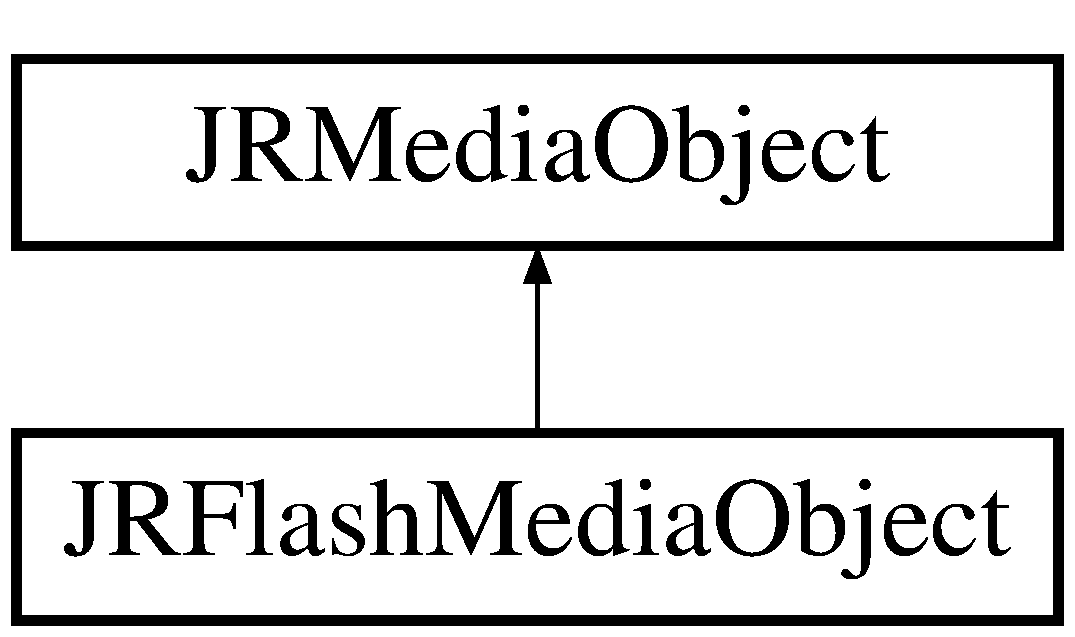
\includegraphics[height=2.000000cm]{interface_j_r_flash_media_object}
\end{center}
\end{figure}
\subsection*{Public Member Functions}
\begin{DoxyCompactItemize}
\item 
(id) -\/ \hyperlink{interface_j_r_flash_media_object_aed4ac7b682373f36379eb81dea041513}{initWithSwfsrc:andImgsrc:}
\end{DoxyCompactItemize}
\subsection*{Properties}
\begin{DoxyCompactItemize}
\item 
NSString $\ast$ \hyperlink{interface_j_r_flash_media_object_a5a79b3d8071ac0286b3ee60e9e0138d0}{swfsrc}
\item 
NSString $\ast$ \hyperlink{interface_j_r_flash_media_object_a5a26cacd216012b37900445a8161ac56}{imgsrc}
\item 
NSUInteger \hyperlink{interface_j_r_flash_media_object_aaeb77e697438b7aa6e44f52bea0ed9c2}{width}
\item 
NSUInteger \hyperlink{interface_j_r_flash_media_object_a0689e19fdf6cb9d3911878a95d6ebcc9}{height}
\item 
NSUInteger \hyperlink{interface_j_r_flash_media_object_a9c380d0410afa60d99442f4ab84b517c}{expanded\_\-width}
\item 
NSUInteger \hyperlink{interface_j_r_flash_media_object_ae390a89405d768f2fcc63c24a8271503}{expanded\_\-height}
\item 
UIImage $\ast$ \hyperlink{interface_j_r_flash_media_object_ac2969bd0da7e91ffa99758dcccb26efb}{preview}
\end{DoxyCompactItemize}


\subsection{Detailed Description}
Flash object to be included in a post to a user's stream. Create an flash media object, fill in the object's fields, and add the object the JRActivity's media array. How the flash videos get presented and whether or not they are used, depend on the provider.

Each video must contain a swfsrc url, which is the URL of the Flash object to be rendered, and an imgsrc, which is the URL of an photo that should be displayed in place of the flash object until the user clicks to prompt the flash object to play. Flash object has two optional fields, {\ttfamily width} and {\ttfamily height}, which can be used to override the default choices when displaying the video in the provider's stream (e.g., Facebook's stream). It also has two optional fields, {\ttfamily expanded\_\-width} and {\ttfamily expanded\_\-height}, to specify the width and height of flash object will resize to, on the provider's stream, once the user clicks on it.

\begin{DoxyNote}{Note}
You can only include one {\ttfamily \hyperlink{interface_j_r_flash_media_object}{JRFlashMediaObject}} in the media array. Any others will be ignored.
\end{DoxyNote}
\begin{DoxySeeAlso}{See also}
Format and rules are identical to those described on the \hyperlink{}{Facebook Developer page on Attachments. } 
\end{DoxySeeAlso}


\subsection{Member Function Documentation}
\hypertarget{interface_j_r_flash_media_object_aed4ac7b682373f36379eb81dea041513}{
\index{JRFlashMediaObject@{JRFlashMediaObject}!initWithSwfsrc:andImgsrc:@{initWithSwfsrc:andImgsrc:}}
\index{initWithSwfsrc:andImgsrc:@{initWithSwfsrc:andImgsrc:}!JRFlashMediaObject@{JRFlashMediaObject}}
\subsubsection[{initWithSwfsrc:andImgsrc:}]{\setlength{\rightskip}{0pt plus 5cm}-\/ (id) initWithSwfsrc: 
\begin{DoxyParamCaption}
\item[{dummy(NSString $\ast$)}]{ \_\-swfsrc}
\item[{andImgsrc:(NSString $\ast$)}]{ \_\-imgsrc}
\end{DoxyParamCaption}
}}
\label{interface_j_r_flash_media_object_aed4ac7b682373f36379eb81dea041513}
Returns a {\ttfamily \hyperlink{interface_j_r_flash_media_object}{JRFlashMediaObject}} initialized with the given swfsrc and imgsrc.


\begin{DoxyParams}{Parameters}
\item[{\em \_\-swfsrc}]The URL of the Flash object to be rendered. This value cannot be {\ttfamily nil}.\item[{\em \_\-imgsrc}]The URL of an photo that should be displayed in place of the flash object. This value cannot be {\ttfamily nil}.\end{DoxyParams}
\begin{DoxyReturn}{Returns}
A {\ttfamily \hyperlink{interface_j_r_flash_media_object}{JRFlashMediaObject}} initialized with the given {\itshape swfsrc\/} and {\itshape imgsrc\/}. If either {\ttfamily \_\-swfsrc} or {\ttfamily \_\-imgsrc} are nil, returns {\ttfamily nil}. 
\end{DoxyReturn}


\subsection{Properties}
\hypertarget{interface_j_r_flash_media_object_a5a79b3d8071ac0286b3ee60e9e0138d0}{
\index{JRFlashMediaObject@{JRFlashMediaObject}!swfsrc@{swfsrc}}
\index{swfsrc@{swfsrc}!JRFlashMediaObject@{JRFlashMediaObject}}
\subsubsection[{swfsrc}]{\setlength{\rightskip}{0pt plus 5cm}-\/ (NSString $\ast$) swfsrc\hspace{0.3cm}{\ttfamily  \mbox{[}read, assign\mbox{]}}}}
\label{interface_j_r_flash_media_object_a5a79b3d8071ac0286b3ee60e9e0138d0}
The URL of the Flash object to be rendered \hypertarget{interface_j_r_flash_media_object_a5a26cacd216012b37900445a8161ac56}{
\index{JRFlashMediaObject@{JRFlashMediaObject}!imgsrc@{imgsrc}}
\index{imgsrc@{imgsrc}!JRFlashMediaObject@{JRFlashMediaObject}}
\subsubsection[{imgsrc}]{\setlength{\rightskip}{0pt plus 5cm}-\/ (NSString $\ast$) imgsrc\hspace{0.3cm}{\ttfamily  \mbox{[}read, assign\mbox{]}}}}
\label{interface_j_r_flash_media_object_a5a26cacd216012b37900445a8161ac56}
The URL of an photo that should be displayed in place of the flash object \hypertarget{interface_j_r_flash_media_object_aaeb77e697438b7aa6e44f52bea0ed9c2}{
\index{JRFlashMediaObject@{JRFlashMediaObject}!width@{width}}
\index{width@{width}!JRFlashMediaObject@{JRFlashMediaObject}}
\subsubsection[{width}]{\setlength{\rightskip}{0pt plus 5cm}-\/ (NSUInteger) width\hspace{0.3cm}{\ttfamily  \mbox{[}read, write, assign\mbox{]}}}}
\label{interface_j_r_flash_media_object_aaeb77e697438b7aa6e44f52bea0ed9c2}
Used to override the default width \hypertarget{interface_j_r_flash_media_object_a0689e19fdf6cb9d3911878a95d6ebcc9}{
\index{JRFlashMediaObject@{JRFlashMediaObject}!height@{height}}
\index{height@{height}!JRFlashMediaObject@{JRFlashMediaObject}}
\subsubsection[{height}]{\setlength{\rightskip}{0pt plus 5cm}-\/ (NSUInteger) height\hspace{0.3cm}{\ttfamily  \mbox{[}read, write, assign\mbox{]}}}}
\label{interface_j_r_flash_media_object_a0689e19fdf6cb9d3911878a95d6ebcc9}
Used to override the default height \hypertarget{interface_j_r_flash_media_object_a9c380d0410afa60d99442f4ab84b517c}{
\index{JRFlashMediaObject@{JRFlashMediaObject}!expanded\_\-width@{expanded\_\-width}}
\index{expanded\_\-width@{expanded\_\-width}!JRFlashMediaObject@{JRFlashMediaObject}}
\subsubsection[{expanded\_\-width}]{\setlength{\rightskip}{0pt plus 5cm}-\/ (NSUInteger) expanded\_\-width\hspace{0.3cm}{\ttfamily  \mbox{[}read, write, assign\mbox{]}}}}
\label{interface_j_r_flash_media_object_a9c380d0410afa60d99442f4ab84b517c}
Width the video will resize to once the user clicks it \hypertarget{interface_j_r_flash_media_object_ae390a89405d768f2fcc63c24a8271503}{
\index{JRFlashMediaObject@{JRFlashMediaObject}!expanded\_\-height@{expanded\_\-height}}
\index{expanded\_\-height@{expanded\_\-height}!JRFlashMediaObject@{JRFlashMediaObject}}
\subsubsection[{expanded\_\-height}]{\setlength{\rightskip}{0pt plus 5cm}-\/ (NSUInteger) expanded\_\-height\hspace{0.3cm}{\ttfamily  \mbox{[}read, write, assign\mbox{]}}}}
\label{interface_j_r_flash_media_object_ae390a89405d768f2fcc63c24a8271503}
Height the video will resize to once the user clicks it \hypertarget{interface_j_r_flash_media_object_ac2969bd0da7e91ffa99758dcccb26efb}{
\index{JRFlashMediaObject@{JRFlashMediaObject}!preview@{preview}}
\index{preview@{preview}!JRFlashMediaObject@{JRFlashMediaObject}}
\subsubsection[{preview}]{\setlength{\rightskip}{0pt plus 5cm}-\/ (UIImage $\ast$) preview\hspace{0.3cm}{\ttfamily  \mbox{[}read, write, retain\mbox{]}}}}
\label{interface_j_r_flash_media_object_ac2969bd0da7e91ffa99758dcccb26efb}
Contains the downloaded preview of the image for display in the publish activity dialog 

The documentation for this class was generated from the following file:\begin{DoxyCompactItemize}
\item 
/Users/lillialexis/iPhone/engage.iphone/JREngage/Classes/\hyperlink{_j_r_activity_object_8h}{JRActivityObject.h}\end{DoxyCompactItemize}

\hypertarget{interface_j_r_image_media_object}{
\section{JRImageMediaObject Class Reference}
\label{interface_j_r_image_media_object}\index{JRImageMediaObject@{JRImageMediaObject}}
}


Image object to be included in a post to a user's stream.  




{\ttfamily \#import $<$JRActivityObject.h$>$}



Inherits JRMediaObject.

\subsection*{Public Member Functions}
\begin{DoxyCompactItemize}
\item 
(id) -\/ \hyperlink{interface_j_r_image_media_object_a8a15f579b784dbdcdaeea9dc1da56cb3}{initWithSrc:andHref:}
\end{DoxyCompactItemize}
\subsection*{Properties}
\begin{DoxyCompactItemize}
\item 
NSString $\ast$ \hyperlink{interface_j_r_image_media_object_aad75823f9189dfca758bc4d4712c3621}{src}
\item 
NSString $\ast$ \hyperlink{interface_j_r_image_media_object_a95642c3f4bc97a112a3ab32beef46f66}{href}
\end{DoxyCompactItemize}


\subsection{Detailed Description}
Image object to be included in a post to a user's stream. Create an image media object, fill in the object's fields, and add the object to the \hyperlink{interface_j_r_activity_object_a2e4ff78f83d0f353f8e0c17ed48ce0ab}{JRActivityObject::media} array in your \hyperlink{interface_j_r_activity_object}{JRActivityObject}. How the images get presented and whether or not they are used, depend on the provider.

Each image must contain a {\itshape src\/} URL, which maps to the photo's URL, and an {\itshape href\/} URL, which maps to the URL where a user should be taken if he or she clicks the photo.

\begin{DoxySeeAlso}{See also}
Format and rules are identical to those described on the \href{http://developers.facebook.com/docs/guides/attachments}{\tt Facebook Developer page on Attachments}. 
\end{DoxySeeAlso}


\subsection{Member Function Documentation}
\hypertarget{interface_j_r_image_media_object_a8a15f579b784dbdcdaeea9dc1da56cb3}{
\index{JRImageMediaObject@{JRImageMediaObject}!initWithSrc:andHref:@{initWithSrc:andHref:}}
\index{initWithSrc:andHref:@{initWithSrc:andHref:}!JRImageMediaObject@{JRImageMediaObject}}
\subsubsection[{initWithSrc:andHref:}]{\setlength{\rightskip}{0pt plus 5cm}-\/ (id) initWithSrc: 
\begin{DoxyParamCaption}
\item[{dummy(NSString $\ast$)}]{ \_\-src}
\item[{andHref:(NSString $\ast$)}]{ \_\-href}
\end{DoxyParamCaption}
}}
\label{interface_j_r_image_media_object_a8a15f579b784dbdcdaeea9dc1da56cb3}
Returns a {\ttfamily \hyperlink{interface_j_r_image_media_object}{JRImageMediaObject}} initialized with the given src and href.


\begin{DoxyParams}{Parameters}
\item[{\em \_\-src}]The photo's URL. This value cannot be {\ttfamily nil}.\item[{\em \_\-href}]The URL where a user should be taken if he or she clicks the photo. This value cannot be {\ttfamily nil}.\end{DoxyParams}
\begin{DoxyReturn}{Returns}
A \hyperlink{interface_j_r_image_media_object}{JRImageMediaObject} initialized with the given src and href. If either {\ttfamily \_\-src} or {\ttfamily \_\-href} are {\itshape nil\/}, returns {\ttfamily nil}. 
\end{DoxyReturn}


\subsection{Properties}
\hypertarget{interface_j_r_image_media_object_aad75823f9189dfca758bc4d4712c3621}{
\index{JRImageMediaObject@{JRImageMediaObject}!src@{src}}
\index{src@{src}!JRImageMediaObject@{JRImageMediaObject}}
\subsubsection[{src}]{\setlength{\rightskip}{0pt plus 5cm}-\/ (NSString $\ast$) src\hspace{0.3cm}{\ttfamily  \mbox{[}read, assign\mbox{]}}}}
\label{interface_j_r_image_media_object_aad75823f9189dfca758bc4d4712c3621}
The photo's URL \hypertarget{interface_j_r_image_media_object_a95642c3f4bc97a112a3ab32beef46f66}{
\index{JRImageMediaObject@{JRImageMediaObject}!href@{href}}
\index{href@{href}!JRImageMediaObject@{JRImageMediaObject}}
\subsubsection[{href}]{\setlength{\rightskip}{0pt plus 5cm}-\/ (NSString $\ast$) href\hspace{0.3cm}{\ttfamily  \mbox{[}read, assign\mbox{]}}}}
\label{interface_j_r_image_media_object_a95642c3f4bc97a112a3ab32beef46f66}
The URL where a user should be taken if he or she clicks the photo. 

The documentation for this class was generated from the following file:\begin{DoxyCompactItemize}
\item 
/Users/lillialexis/iPhone/engage.iphone/JREngage/Classes/\hyperlink{_j_r_activity_object_8h}{JRActivityObject.h}\end{DoxyCompactItemize}

\hypertarget{interface_j_r_mp3_media_object}{
\section{JRMp3MediaObject Class Reference}
\label{interface_j_r_mp3_media_object}\index{JRMp3MediaObject@{JRMp3MediaObject}}
}


Mp3 object to be included in a post to a user's stream.  




{\ttfamily \#import $<$JRActivityObject.h$>$}



Inherits JRMediaObject.

\subsection*{Properties}
\begin{DoxyCompactItemize}
\item 
NSString $\ast$ \hyperlink{interface_j_r_mp3_media_object_ae6ae676c1841834aba74a2c5d11cb54c}{src}
\item 
NSString $\ast$ \hyperlink{interface_j_r_mp3_media_object_accd252e22f704fd4b314217317f0b5cb}{title}
\item 
NSString $\ast$ \hyperlink{interface_j_r_mp3_media_object_aa164b3ecc14b03d36f5093d3d4d7f5b1}{artist}
\item 
NSString $\ast$ \hyperlink{interface_j_r_mp3_media_object_adefc6578183aa09a492b229696f581df}{album}
\end{DoxyCompactItemize}
\subsection*{Constructors}
\label{_amgrp559a25fdb98a7d1fd1c3771ac568d5e9}
 \begin{DoxyCompactItemize}
\item 
(id) -\/ \hyperlink{interface_j_r_mp3_media_object_a15eba85b9094d28d8d9bc6b9625ee55c}{initWithSrc:}
\item 
(id) + \hyperlink{interface_j_r_mp3_media_object_ab8788e64a6d5b868e1b0689d55d68246}{mp3MediaObjectWithSrc:}
\end{DoxyCompactItemize}


\subsection{Detailed Description}
Mp3 object to be included in a post to a user's stream. Create an mp3 media object, fill in the object's fields, and add the object to the \hyperlink{interface_j_r_activity_object_a2e4ff78f83d0f353f8e0c17ed48ce0ab}{JRActivityObject::media} array in your \hyperlink{interface_j_r_activity_object}{JRActivityObject}. How the mp3s get presented and whether or not they are used, depend on the provider.

Each mp3 must contain a {\itshape src\/} url, which is the URL of the MP3 file to be rendered. The mp3 can also include a {\itshape title\/}, {\itshape artist\/}, and {\itshape album\/}.

\begin{DoxyNote}{Note}
You can only include one \hyperlink{interface_j_r_mp3_media_object}{JRMp3MediaObject} in the media array. Any others will be ignored.
\end{DoxyNote}
\begin{DoxySeeAlso}{See also}
Format and rules are identical to those described on the \href{http://developers.facebook.com/docs/guides/attachments}{\tt Facebook Developer page on Attachments}. 
\end{DoxySeeAlso}


\subsection{Member Function Documentation}
\hypertarget{interface_j_r_mp3_media_object_a15eba85b9094d28d8d9bc6b9625ee55c}{
\index{JRMp3MediaObject@{JRMp3MediaObject}!initWithSrc:@{initWithSrc:}}
\index{initWithSrc:@{initWithSrc:}!JRMp3MediaObject@{JRMp3MediaObject}}
\subsubsection[{initWithSrc:}]{\setlength{\rightskip}{0pt plus 5cm}-\/ (id) initWithSrc: 
\begin{DoxyParamCaption}
\item[{dummy(NSString $\ast$)}]{ \_\-src}
\end{DoxyParamCaption}
}}
\label{interface_j_r_mp3_media_object_a15eba85b9094d28d8d9bc6b9625ee55c}
Returns a {\ttfamily \hyperlink{interface_j_r_mp3_media_object}{JRMp3MediaObject}} initialized with the given src.


\begin{DoxyParams}{Parameters}
\item[{\em \_\-src}]The URL of the MP3 file to be rendered. This value cannot be {\ttfamily nil}.\end{DoxyParams}
\begin{DoxyReturn}{Returns}
A \hyperlink{interface_j_r_mp3_media_object}{JRMp3MediaObject} initialized with the given src. If {\ttfamily \_\-src} is {\itshape nil\/}, returns {\ttfamily nil}. 
\end{DoxyReturn}
\hypertarget{interface_j_r_mp3_media_object_ab8788e64a6d5b868e1b0689d55d68246}{
\index{JRMp3MediaObject@{JRMp3MediaObject}!mp3MediaObjectWithSrc:@{mp3MediaObjectWithSrc:}}
\index{mp3MediaObjectWithSrc:@{mp3MediaObjectWithSrc:}!JRMp3MediaObject@{JRMp3MediaObject}}
\subsubsection[{mp3MediaObjectWithSrc:}]{\setlength{\rightskip}{0pt plus 5cm}+ (id) mp3MediaObjectWithSrc: 
\begin{DoxyParamCaption}
\item[{dummy(NSString $\ast$)}]{ \_\-src}
\end{DoxyParamCaption}
}}
\label{interface_j_r_mp3_media_object_ab8788e64a6d5b868e1b0689d55d68246}
Returns a {\ttfamily \hyperlink{interface_j_r_mp3_media_object}{JRMp3MediaObject}} initialized with the given src.


\begin{DoxyParams}{Parameters}
\item[{\em \_\-src}]The URL of the MP3 file to be rendered. This value cannot be {\ttfamily nil}.\end{DoxyParams}
\begin{DoxyReturn}{Returns}
A \hyperlink{interface_j_r_mp3_media_object}{JRMp3MediaObject} initialized with the given src. If {\ttfamily \_\-src} is {\itshape nil\/}, returns {\ttfamily nil}. 
\end{DoxyReturn}


\subsection{Properties}
\hypertarget{interface_j_r_mp3_media_object_ae6ae676c1841834aba74a2c5d11cb54c}{
\index{JRMp3MediaObject@{JRMp3MediaObject}!src@{src}}
\index{src@{src}!JRMp3MediaObject@{JRMp3MediaObject}}
\subsubsection[{src}]{\setlength{\rightskip}{0pt plus 5cm}-\/ (NSString $\ast$) src\hspace{0.3cm}{\ttfamily  \mbox{[}read, assign\mbox{]}}}}
\label{interface_j_r_mp3_media_object_ae6ae676c1841834aba74a2c5d11cb54c}
The URL of the MP3 file to be rendered \hypertarget{interface_j_r_mp3_media_object_accd252e22f704fd4b314217317f0b5cb}{
\index{JRMp3MediaObject@{JRMp3MediaObject}!title@{title}}
\index{title@{title}!JRMp3MediaObject@{JRMp3MediaObject}}
\subsubsection[{title}]{\setlength{\rightskip}{0pt plus 5cm}-\/ (NSString $\ast$) title\hspace{0.3cm}{\ttfamily  \mbox{[}read, write, retain\mbox{]}}}}
\label{interface_j_r_mp3_media_object_accd252e22f704fd4b314217317f0b5cb}
The title of the song \hypertarget{interface_j_r_mp3_media_object_aa164b3ecc14b03d36f5093d3d4d7f5b1}{
\index{JRMp3MediaObject@{JRMp3MediaObject}!artist@{artist}}
\index{artist@{artist}!JRMp3MediaObject@{JRMp3MediaObject}}
\subsubsection[{artist}]{\setlength{\rightskip}{0pt plus 5cm}-\/ (NSString $\ast$) artist\hspace{0.3cm}{\ttfamily  \mbox{[}read, write, retain\mbox{]}}}}
\label{interface_j_r_mp3_media_object_aa164b3ecc14b03d36f5093d3d4d7f5b1}
The artist \hypertarget{interface_j_r_mp3_media_object_adefc6578183aa09a492b229696f581df}{
\index{JRMp3MediaObject@{JRMp3MediaObject}!album@{album}}
\index{album@{album}!JRMp3MediaObject@{JRMp3MediaObject}}
\subsubsection[{album}]{\setlength{\rightskip}{0pt plus 5cm}-\/ (NSString $\ast$) album\hspace{0.3cm}{\ttfamily  \mbox{[}read, write, retain\mbox{]}}}}
\label{interface_j_r_mp3_media_object_adefc6578183aa09a492b229696f581df}
The album 

The documentation for this class was generated from the following file:\begin{DoxyCompactItemize}
\item 
/Users/lillialexis/iPhone/engage.iphone/JREngage/Classes/\hyperlink{_j_r_activity_object_8h}{JRActivityObject.h}\end{DoxyCompactItemize}

\chapter{File Documentation}
\hypertarget{_j_r_activity_object_8h}{
\section{/Users/lillialexis/iPhone/engage.iphone/JREngage/Classes/JRActivityObject.h File Reference}
\label{_j_r_activity_object_8h}\index{/Users/lillialexis/iPhone/engage.iphone/JREngage/Classes/JRActivityObject.h@{/Users/lillialexis/iPhone/engage.iphone/JREngage/Classes/JRActivityObject.h}}
}


Interface for creating and populating activities that you wish to publish.  


{\ttfamily \#import $<$Foundation/Foundation.h$>$}\par
{\ttfamily \#import \char`\"{}JRConnectionManager.h\char`\"{}}\par
\subsection*{Classes}
\begin{DoxyCompactItemize}
\item 
class \hyperlink{interface_j_r_image_media_object}{JRImageMediaObject}
\begin{DoxyCompactList}\small\item\em Image object to be included in a post to a user's stream. \item\end{DoxyCompactList}\item 
class \hyperlink{interface_j_r_flash_media_object}{JRFlashMediaObject}
\begin{DoxyCompactList}\small\item\em Flash object to be included in a post to a user's stream. \item\end{DoxyCompactList}\item 
class \hyperlink{interface_j_r_mp3_media_object}{JRMp3MediaObject}
\begin{DoxyCompactList}\small\item\em Mp3 object to be included in a post to a user's stream. \item\end{DoxyCompactList}\item 
class \hyperlink{interface_j_r_action_link}{JRActionLink}
\begin{DoxyCompactList}\small\item\em A link a user can use to take action on an activity update on the provider. \item\end{DoxyCompactList}\item 
class \hyperlink{interface_j_r_activity_object}{JRActivityObject}
\begin{DoxyCompactList}\small\item\em An activity object you create, populate, and post to the user's activity stream. \item\end{DoxyCompactList}\end{DoxyCompactItemize}


\subsection{Detailed Description}
Interface for creating and populating activities that you wish to publish. Interface for creating and populating activities that you wish to publish to your user's social networks. Create an activity object, fill in the object's fields, and pass the object to the \hyperlink{interface_j_r_engage}{JREngage} library when you are ready to share. 
\printindex
\end{document}
